\documentclass[12pt,]{article}
\usepackage{lmodern}
\usepackage{amssymb,amsmath}
\usepackage{ifxetex,ifluatex}
\usepackage{fixltx2e} % provides \textsubscript
\ifnum 0\ifxetex 1\fi\ifluatex 1\fi=0 % if pdftex
  \usepackage[T1]{fontenc}
  \usepackage[utf8]{inputenc}
\else % if luatex or xelatex
  \ifxetex
    \usepackage{mathspec}
  \else
    \usepackage{fontspec}
  \fi
  \defaultfontfeatures{Ligatures=TeX,Scale=MatchLowercase}
\fi
% use upquote if available, for straight quotes in verbatim environments
\IfFileExists{upquote.sty}{\usepackage{upquote}}{}
% use microtype if available
\IfFileExists{microtype.sty}{%
\usepackage{microtype}
\UseMicrotypeSet[protrusion]{basicmath} % disable protrusion for tt fonts
}{}
\usepackage[letterpaper, left = 1in, right = 1in, top = 1.5in, bottom = 1.5in]{geometry}
\usepackage{hyperref}
\hypersetup{unicode=true,
            pdftitle={Financialization of Commodities: an Asset Pricing Perspective},
            pdfkeywords={Commodity futures; financialization; hedging pressure; financial crisis},
            pdfborder={0 0 0},
            breaklinks=true}
\urlstyle{same}  % don't use monospace font for urls
\usepackage{natbib}
\bibliographystyle{jf}
\usepackage{graphicx,grffile}
\makeatletter
\def\maxwidth{\ifdim\Gin@nat@width>\linewidth\linewidth\else\Gin@nat@width\fi}
\def\maxheight{\ifdim\Gin@nat@height>\textheight\textheight\else\Gin@nat@height\fi}
\makeatother
% Scale images if necessary, so that they will not overflow the page
% margins by default, and it is still possible to overwrite the defaults
% using explicit options in \includegraphics[width, height, ...]{}
\setkeys{Gin}{width=\maxwidth,height=\maxheight,keepaspectratio}
\IfFileExists{parskip.sty}{%
\usepackage{parskip}
}{% else
\setlength{\parindent}{0pt}
\setlength{\parskip}{6pt plus 2pt minus 1pt}
}
\setlength{\emergencystretch}{3em}  % prevent overfull lines
\providecommand{\tightlist}{%
  \setlength{\itemsep}{0pt}\setlength{\parskip}{0pt}}
\setcounter{secnumdepth}{5}
% Redefines (sub)paragraphs to behave more like sections
\ifx\paragraph\undefined\else
\let\oldparagraph\paragraph
\renewcommand{\paragraph}[1]{\oldparagraph{#1}\mbox{}}
\fi
\ifx\subparagraph\undefined\else
\let\oldsubparagraph\subparagraph
\renewcommand{\subparagraph}[1]{\oldsubparagraph{#1}\mbox{}}
\fi

%%% Use protect on footnotes to avoid problems with footnotes in titles
\let\rmarkdownfootnote\footnote%
\def\footnote{\protect\rmarkdownfootnote}


  \title{Financialization of Commodities: an Asset Pricing Perspective}
    % \author{Devraj Basu \\ Olivier Bauthéac}
  \author{ Devraj Basu  \\  Olivier Bauthéac  
	  \thanks{ Basu: University of Strathclyde, Glasgow, UK, \href{mailto:devraj.basu@strath.ac.uk}{\nolinkurl{devraj.basu@strath.ac.uk}}.  Bauthéac: University of Strathclyde, Glasgow, UK, \href{mailto:olivier.bautheac@strath.ac.uk}{\nolinkurl{olivier.bautheac@strath.ac.uk}}. 	  
	   \newline We thank seminar participants at IIM Ahmedabad, IIM Calcutta, SKEMA
Business School and University of Gottingen, as well as Griffith
inaugural alternative investment conference attendants for their
feedback. We also thank Joelle Miffre, Martijn Boons, John Fan, Robert
Bianchi, Chardin Wese Simen, Andrew Kaleel and particularly Olaf Korn
for their extremely useful comments and suggestions.  }
  }
    \date{}
  
\usepackage{longtable, tabu, pdflscape, booktabs, caption, setspace}
\doublespacing
\renewcommand*{\arraystretch}{0.65}


\begin{document}
\maketitle
\begin{abstract}
The last two decades have seen major changes in the nature of the
commodity markets with the influx of financial investor inflows followed
by the financial crisis. We study the effect of these events on
commodity futures pricing dynamics using commodity asset pricing
techniques. We find that a non-price based factor is best able to detect
the effects of commodity financialization, while the effects of the
financial crisis and after are most clearly visible through the
performance of the market factor. The effects of financialization seem
to go beyond mechanical effects induced by the rise of indexing. 
\newline
JEL: G11, G23, G13, Q02
\newline
Keywords: Commodity futures, financialization, hedging pressure, financial crisis

\end{abstract}


\newpage

\textbf{Disclosure}

\begin{itemize}
\tightlist
\item
  Devraj Basu: I am a co-author of this paper and wish to state that I
  have no conflict of interest, financial or otherwise. I do not hold
  paid or unpaid positions at any organization whose goals relate to the
  article.\\
  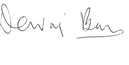
\includegraphics{pics/signature - Devraj.png}\\
\end{itemize}

\newpage

\textbf{Disclosure}

\begin{itemize}
\tightlist
\item
  Olivier Bauthéac: I am a co-author of this paper and wish to state
  that I have no conflict of interest, financial or otherwise. I do not
  hold paid or unpaid positions at any organization whose goals relate
  to the article.\\
  
\includegraphics{pics/signature - Olivier.png}\\
\end{itemize}

\newpage

\hypertarget{introduction}{%
\section{Introduction}\label{introduction}}

The last twenty years have seen major upheavals in the commodity markets
with the onset of financialization\footnote{Starting around 2004, with a
  view of commodity markets as an emerging asset class and in an effort
  to hedge against inflation and seek diversification benefits
  \citep{buyuksahin_speculators_2014, singleton_investor_2013},
  institutional investors sent forth an unprecedented flow of capital
  into commodity futures markets. This phenomenon is commonly referred
  to as the financialization of commodities
  \citep{domanski_financial_2007}.} as well as the period of the 2008
financial crisis and its aftermath. Financialization appears to have
affected a number of economic sectors, including agriculture and energy,
and its impact has been hotly debated in the policy, legislative,
regulatory, and academic spheres. A vigorous legislative debate has led
to regulatory changes accompanied by an equally intense policy and
academic debate across a number of disciplines about the perceived
effects on commodity prices of the unprecedented inflow of institutional
funds brought into commodity futures markets by new index type
investors\footnote{See section \ref{background} for a detailled
  discussion.}. In response to immediate policy concerns, the academic
debate was initially framed rather narrowly. In this paper we take a
fundamentally different empirical approach that is broader in scope. We
consider the entire cross-section of actively traded commodities on
futures markets and use a futures based asset pricing framework that
includes factors constructed using both price and non-price attributes.

Commodity futures markets have a history of being the classic physical
commodity risks shifting conduit for commodity specialists, and
financialization may have altered this long standing paradigm with the
entry of long only commodity index traders (CITs) with very different
hedging and volume demands from traditional participants. This change
could have altered the hedging ontology in these markets and our asset
pricing framework is well suited to detect these more subtle effects
driven by changes in the nature of traders. Factor model techniques are
well suited to isolating common driving factors and detecting
co-movement and building on theory we develop a bespoke commodity-based
asset pricing framework that seems well adapted to study these two
issues simultaneously.

The first factor model we consider (CHP) is based on the well-known
hedging pressure based theory
\citep{anderson_hedger_1983, chang_returns_1985, cootner_returns_1960, dusak_futures_1973, hicks_value_1939, hirshleifer_risk_1988, hirshleifer_determinants_1989, hirshleifer_hedging_1990, kolb_is_1992, keynes_treatise_1930}
which postulates that futures prices for a given commodity are inversely
related to the extent that commercial hedgers are short or long and we
use a factor mimicking portfolio that captures the impact of hedging
pressure as a systemic factor \citep{basu_capturing_2013}. Our second
factor model is based on open interest growth following
\citet{hong_what_2012} who find that open interest growth has predictive
power for individual commodity returns and again we construct a
long-short factor mimicking portfolio. Our third model is based on term
structure following \citet{szymanowska_anatomy_2014} and
\citet{fuertes_commodity_2015} who demonstrate that the term structure
factor has explanatory power for the cross-section of commodity returns.
We finally consider an equally weighted portfolio of commodities as a
proxy for the market factor. Our two price based and two non-price based
factors allow us to compare and contrast different channels that could
have led to changes in commodity price dynamics over the last twenty
years.

We study the performance of these models on a set of twenty-four US
traded commodities and six UK traded (LME exchange) base metals over the
1997/2017 period that we divide into four distinct sub-periods. The
first, the pre-financialization phase, spans the 1997/2003 period; the
second, the financialization phase, spans the 2004/2007 period\footnote{Starting
  point based on earlier studies
  \citep{baker_financialization_2014, christoffersen_factor_2014}.}; the
third, 2008/2013, encompasses both the financial crisis and the loose
monetary policy regimes that followed; and the fourth spans the period
starting in 2014 to present.\\
Consistent with earlier studies, we observe that mean returns for the US
traded commodities are sharply higher over the financialization period
compared to pre-financialization and this pattern extends to UK traded
metals.

The cross-sectional nature of financialization
\citep{basak_model_2016, cheng_financialization_2014} leads us to extend
the Keynesian individual hedging pressure paradigm by incorporating
aggregate CHP (\textbf{CHP}), a market wide measure of hedging pressure
first considered in \citet{hong_what_2012}. This paradigm implies that
returns for individual commodities should be high in periods where
\textbf{CHP} is low (\textbf{backwardation}) and low in periods where
\textbf{CHP} is high (\textbf{contango}). Over the first period the
cross sectional average returns during \textbf{backwardation} for both
the US and UK commodities are positive with those for the US
statistically significant, and significantly higher than during
\textbf{contango}, providing broad support for an aggregate version of
the Keynesian hedging pressure hypothesis. Over the second period this
pattern reverses, with both the US and UK commodities having significant
positive returns during \textbf{contango} with these returns being
significantly higher than during \textbf{backwardation}. This change in
pattern suggests that the onset of financialization altered the
traditional risk shifting nature of hedger's behaviour, which is implied
by the Keynesian hypothesis. The arrival of financial investors raises
the question of whether they functioned as liquidity providers or
liquidity demanders. Arguments have been made for both of these
possibilities with \citet{moskowitz_time_2012} arguing that financial
investors provide liquidity while \citet{Kangtaletwopremiums2017} argue
that they demand liquidity. Our analysis of returns in periods of low
and high aggregate CHP before and during financialization allows us to
analyse this issue from a new perspective and suggests that financial
investors may have been liquidity demanders leading hedgers to become
liquidity providers.

\citet{goldstein_commodity_2017} as well as
\citet{goldstein_speculation_2014} argue that the arrival of financial
investors has an impact on the extent of normal backwardation in
commodity futures markets. Based on their analysis we would expect our
average CHP factor, which is based on backwardation measured by hedger's
positions, as well our term structure factor, which is based on
backwardation measured by roll yield, to be best suited to measure the
impact of financialization.\\
We analyze the pricing dynamics over the different periods by first
studying the time series pricing performance of the various factors on
all the US traded commodities with the factors constructed using the
latter set of commodities. The market based factor outperforms the other
three in the first period and it has a similar level of performance in
the second period, while the CHP factor shows the greatest improvement
in performance in the second period. The performance of the market
factor is driven by agricultural commodities and metals in both the
first and second period and the dramatic improvement of the CHP factor
in the second period is driven by precious and precious-base metals. The
best performing commodities for the market factor exhibited
approximately the same level of price co-movement both before and during
financialization. In contrast, the best performing commodities for the
CHP factor exhibited very low pair-wise correlation in the first period,
around the average for US traded commodities, while during
financialization the average pairwise correlation between the top
performing CHP factor commodities is higher than that for the market
factor and double of the average for all the US traded commodities. This
increase is due to the dramatic rise in average pairwise correlation
amongst the US traded metals all of which exhibited high
R\textsuperscript{2} with respect to the CHP factor during
financialization which in turn is due to their common low level of CHP
over this period. Thus the CHP factor model is able to establish the
strengthening link between a non-price attribute and price dynamics in
the US metal sub-sector during financialization.\\
We explore this issue further by constructing the four factors with the
top eight commodities for a given factor (factor picks) in each
period\footnote{See section \ref{methods} for further details.} and
evaluating its performance on these selected commodities as well as on
all US traded commodities. The results of this exercise strongly suggest
that the hedging pressure co-movement and price co-movement link was
concentrated in the metals sub-sector.

The UK traded base metals provide a useful set of assets to test how
widespread were the changes in pricing dynamics brought about by the
onset of financialization. To that end, we examine the performance of
the four factors on the six UK metals, when constructed from each set of
factor picks. The resuslts show that here was co-movement in global
metals returns in the second period and that this co-movement could be
detected by our hedging pressure based model.

The onset of the financial crisis and the monetary policy regimes that
followed, on the other hand, also appear to have induced significant
changes in pricing dynamics. Returns on both US and UK traded
commodities fell dramatically over both the third and fourth periods
with the pattern of return for the US traded commodities across
\textbf{CHP} regimes reverting to Keynesian paradigm. The pricing
results indicate the emergence of a systematic factor across the entire
cross-section of the US commodities as well as strong evidence of
cross-market linkages.

Financialization was an issue of such policy importance that it
triggered legislative action. The debate was initially framed around
adequacy of speculation, the burning issue of the day, and the
consequent analysis focused on the more mechanical effects of
financialization. With the benefit of hindsight, it appears this
approach was perhaps too narrow and it now seems necessary to address
financialization from a broader perspective. Commodity price dynamics
appear to have altered substantially in quite different ways over the
financialization and the financial crisis periods and our commodity
futures based asset pricing approach seems able to provide new insights
into the nature of these changes: financialization was a phenomenon
endogenous to the commodity markets transmitted via the commodity
futures markets and mainly concentrated in a specific sector (metals)
while the crisis and its aftermath seems to have delivered an exogenous
shock across the entire cross-section of global commodities. The initial
view of financialization was that it consisted of speculative flows
which had the effect of driving up and creating bubble like conditions
in commodity future prices\footnote{\citet{de_schutter_food_2010_1};
  \citet{gilbert_how_2010}; \citet{gilbert_speculative_2010};
  \citet{masters_testimony_2008}; \citet{masters_accidental_2008};
  \citet{herman_not_2011_1}; \citet{schumann_hunger-makers_2011};
  \citet{singleton_investor_2013}; \citet{unctad_global_2009}.}.
However, the fundamental question of the nature of the impact of
financialization across the entire cross-section of commodity futures
markets has not yet been completely answered. We provide an empirical
complement to a new stream of theoretical studies that try to model the
impact of financialization on various aspects of commodity futures
markets\footnote{\citet{etula_broker-dealer_2013},
  \citet{acharya_limits_2013}, \citet{cheng_convective_2014},
  \citet{leclercq_equilibrium_2014}, \citet{sockin_informational_2015},
  \citet{goldstein_speculation_2013},
  \citet{EkelandSpeculationcommodityfutures2016},
  \citet{goldstein_commodity_2017}.} and demonstrate that the effects of
financialization extend beyond the mechanical effects induced by
indexation as outlined in \citet{basak_model_2016} as well as
\citet{tang_index_2012}.

\hypertarget{data-methods}{%
\section{Data \& methods}\label{data-methods}}

\hypertarget{background}{%
\subsection{Background}\label{background}}

The period from 1998 to 2008 saw an influx of investment into commodity
index linked products most of which made its way into the commodity
futures market. These commodity indexes whose goal was to track the
broad movement of commodity prices could be accessed by means of
exchange traded funds and exchange traded notes. At least \$100 billion
of new investment flowed into these products over the 1998-2008 period
with this financialization phenomenon leading to substantial legislative
changes. Concerns over the consequences of financialization were behind
Rule 76 FR 4752 issued by the US Commodity Futures Trading Commission
(CFTC) on January 26\textsuperscript{th}, 2011. This provision emanates
from the Dodd-Frank Wall Street and Consumer Protection Act of 2010
(Title VII, Section 737) that mandates the CFTC to use position limits
to restrict the flow of speculative capital into a number of commodity
markets. The Rule was approved in a close 3-2 vote and the ensuing
rulemaking process was extremely contentious with several commissioners
(Michael Dunn and Scott D. O'Malia in particular) expressing
reservations about the lack of supporting evidence and the Rule also
triggering thousands of comment letters as well as a lawsuit against the
CFTC spearheaded by two Wall Street trade groups, the International
Swaps \& Derivatives Association (ISDA) and the Securities Industries \&
Financial Markets Association (SIFMA)\footnote{ISDA \& SIFMA v US CFTC;
  Complaint, 1:11-cv-02146; December 2\textsuperscript{nd}, 2011.}.

A world-wide debate has ensued about the role of index funds in
commodity markets. The first responses to the 2007/2008 crisis of
escalating food and energy prices took the form of policy reports, many
of which reasoned that the growth of commodity index funds came along
with an influx of largely speculative capital that was responsible for
driving commodity prices beyond their historic highs
\citep{de_schutter_food_2010_1, gilbert_speculative_2010, herman_not_2011_1, schumann_hunger-makers_2011, unctad_global_2009}.
The US and various european countries also became involved in this
issue. Early US Senate investigations drew on pricing and trading data
supplied by the CFTC as well as interviews with numerous experts
including hedge fund manager Michael Masters who linked the growing
presence of index investors in US wheat markets to the observed surges
in both futures and cash prices
\citep{masters_testimony_2008, masters_accidental_2008}). This
contention has since come to be known as the Masters' hypothesis and was
largely endorsed by the final US Senate report on the issue
\citep{USSenate_Excessive_speculation_wheat_2009}. At this stage, the
question thrust on the academic sphere was whether ``excessive
speculation'' (understood as the market activity peculiar to index type
investors) was linked to escalating energy and agricultural commodity
prices. A number of academic studies, most of which used commodity
specific causality and correlation based analysis have disproved this
contention, particularly in the case of agricultural and energy
commodities. \citet{irwin_devil_2009}, \citet{sanders_adequacy_2010},
\citet{sanders_impact_2011}, \citet{sanders_new_2011},
\citet{irwin_commodity_2013}, \citet{brunetti_commodity_2014},
\citet{hamilton_effects_2015} and \citet{bruno_financialization_2017}
study the agricultural markets. \citet{buyuksahin_speculators_2011},
\citet{tokic_speculation_2012}, \citet{fattouh_role_2013},
\citet{kilian_role_2014}, \citet{knittel_simple_2016} and
\citet{manera_modelling_2016} study the energy markets.
\citet{bohl_does_2013_2}, \citet{kim_does_2015} and
\citet{boyd_prevalence_2016} study both energy and agricultural markets
while \citet{irwin_index_2011}, \citet{irwin_financialization_2012} and
\citet{stoll_commodity_2011} study the commodity markets in general.

Other studies have underlined various alterations in commodity pricing
dynamics over the period. \citet{gilbert_role_2014} reject the view that
financialization has not had any effects in the grains markets and
demonstrate that trades originated by financial actors, and specifically
index investors, can move prices but tend typically to be
volatility-reducing. \citet{cheng_financialization_2014} show that in
the case of index commodities, financialization has transformed the risk
sharing, and information discovery functions of commodity futures
markets. \citet{juvenal_speculation_2015} contend that the oil price
increase between 2004 and 2008 was mainly driven by the strength of
global demand but that the financialization process of commodity markets
also played a role. \citet{henderson_new_2015} show that
non-information-based financial investments have important impacts on
commodity prices.

\hypertarget{data}{%
\subsection{Data}\label{data}}

Commodity index funds (CIFs), commodity based exchange traded funds
(ETFs) and notes (ETNs) as well as commodity linked notes (CLNs) were
amongst the main investment vehicules that allowed institutional and
retail investors to build up commodity exposure in the early 2000s
\citep{boons_stock_2012, henderson_new_2015, irwin_index_2011, unctad_global_2009, schumann_hunger-makers_2011}.
Most of these products were primarily designed to track prominent
commodity indexes amongst which the S\&P-GSCI, the most popular. Most of
its constituents at the time of writting form the basis of the broad
cross-section of commodities that we consider in this study\footnote{See
  section \ref{assets} for details on the commodity pool considered.}.
Unleaded gasoline, the NYMEX legacy contract for gasoline stopped
trading in 2006 when it was replaced by Reformulated Gasoline Blendstock
for Oxygen Blending (RBOB) with the two futures series trading alongside
for most of the year. For our NYMEX gasoline data series, we consider
unleaded gasoline up to September 1\textsuperscript{st}, 2006 and RBOB
gasoline thereafter, date at which liquidity for the latter overtook
that for the former.

The commodity futures trading commission (CFTC) operates a comprehensive
system of collecting information on market participants known as the
large trader reporting program (LTRP) where it records and reports to
the public market position data on market particpants who have position
levels in excess of a particular futures market specific
threshold\footnote{Current reporting level thresholds available at:
  \href{https://www.ecfr.gov/cgi-bin/retrieveECFR?gp=\&SID=970471b8455f4bab7db4110cfde50731\&mc=true\&r=SECTION\&n=se17.1.15_103}{www.ecfr.gov}.}.
The commission collects market data and position information daily from
clearing members, futures commission merchants (FCMs) and foreign
brokers and publishes corresponding summaries weekly in a series of
market specific reports. In these reports, individual traders are
categorised according to the nature of their trading activity on the
basis of self-reported information\footnote{CFTC form 40. Available at:
  \href{https://www.cftc.gov/sites/default/files/idc/groups/public/@forms/documents/file/cftcform40.pdf}{www.cftc.gov}.}
that is subject to review by CFTC staff for reasonableness. Position
information is then aggregated by category and asset type with each
report providing an aggregation for a set of report specific categories
and, for each category, a breakdown between futures only positions and
positions in futures and options combined.\\
In its legacy report, the commitment of trader report (COT) with data
dating back to 1962, the CFTC distinguishes ``commercial'' and
``non-commercial'' market participants where a ``commercial''
participant is defined as one ``{[}\ldots{}{]} engaged in business
activities hedged by the use of futures and option markets''\footnote{See
  \href{https://www.gpo.gov/fdsys/pkg/CFR-1998-title17-vol1/xml/CFR-1998-title17-vol1-sec1-3.xml}{CFTC
  regulation 1.3, 17 CFR 1.3(z)} for details.}. A third category,
``non-reportable'', aggregates positions for participants not meeting
the reporting threshold. In response to concerns related to category
accuracy\footnote{See for example \citet{ederington_who_2002}.} the CFTC
now refines its classification in the disaggregated commitment of trader
report (DCOT) where participant categories include
``Producer/Merchant/Processor/User'', ``Swap dealer'', ``Money manager''
and ``Other reportable'' as well as in the supplemental commitment of
trader report (SCOT) that details commodity index trader aggregate
positions for thirteen agricultural commodity futures markets. Data for
DCOT and SCOT dates back to 2006 and 2007 respectively.\\
We study the 1997/2017 period where we observe futures only position
data from the COT report, the only CFTC report with data available for
the whole period of interest; as well as futures term structure price
and open interest data from Bloomberg.

\hypertarget{methods}{%
\subsection{Methods}\label{methods}}

On the one hand, futures markets have a long history of serving
commodity producers to allievate their commodity price and output risks.
\citet{keynes_treatise_1930} and \citet{hicks_value_1939} emphasise the
``normal'' behaviour of naturally short hedgers outsourcing their
commodity risk to naturally long commodity specialist speculators. This
market configuration is referred to as ``backwardation'' where futures
is expected to trade at a discount to spot, providing speculators with
incentives to take the long side. The opposite market paradigm is
referred to as ``contango''. Working
\citep{working_theory_1948, working_hedging_1953} and Cootner
\citep{cootner_returns_1960, CootnerSpeculationhedging1967} somehow
relax this ``supply-of-speculative-services''
\citep{Tilllongtermperspectivecommodity2007} approach by introducing
processors and merchants, also commodity experts, on the hedgers side
and relating the notions of backwardation and contango more directly to
the term structure via the theory of storage where the shape of the
front end of the term structure (basis) is directly related to the
market price of storage.\\
Financialization, on the other hand, refers to the entry of financial
investors into the commodity futures markets who, for the most part, are
not commodity experts. Besides, these new market participants tend to
exhibit herding like behaviour, often taking massive long-only positions
on the whole cross-section of indexed commodities in an attempt to hedge
against inflation and/or seek further diversification benefits for
portfolios with, in most cases, existing large positions across various
asset classes
\citep{brunetti_speculators_2016, boyd_prevalence_2016, cheng_convective_2014, juvenal_speculation_2015, singleton_investor_2013, tang_index_2012}.
This contrasts with the traditional approaches of Keynes and Working and
in this context the issues of co-movement and aggregate market
participants behaviour seem particularly relevant.\\
Asset pricing techniques are well suited to study co-movement. Building
on theory we develop an ad-hoc commodity based asset pricing framework
that we believe is well adapted to study these two issues simultaneously
and implement it over four periods of interest. The first, the
pre-financialization period, starts in 1997 and is naturally followed by
financialization, spanning the 2004/2007 period, and the financial
crisis and its aftermath, spanning the 2008/2013 period. The last period
spans the 2014/present period sarting with the beginning of the
tapering/end of the US Quantitative Easing program (QE).\\
Using the weekly price, open interest and market position data described
above we construct market portfolios of commodity nearby futures as well
as mimicking portfolios for market, commercial hedging pressure, term
structure and liquidity risk factors in returns. While our market
portfolios are long only, equally weighted portfolios of particular
commodity sets, our other mimicking portfolios for risk factors are
constructed as combinations of two sub-portfolios (legs), one held long,
one held short, which respective constituents are pooled on a weekly
basis according to risk factor specific criterias. The weekly return for
a particular mimicking portfolio is calculated as the difference between
the average return for constituents of the long portfolio and that for
the constituents of the short portfolio. i.e, return on the mimicking
portfolio for risk factor \(i\) (\(f_{i}\)) for week \(t\):

\[r_{t}^{f_{i}}=\frac{1}{x}\sum_{j=1}^{x}r_{j,t}-\frac{1}{x}\sum_{j=n-x}^{n}r_{j,t}\]
\(n\equiv\) number of commodities in the set considered for mimicking
portfolio construction.\\
\(x = \left \lceil n \cdot s \right \rceil\)\\
\(s\equiv\) selection threshold (\(\frac{1}{3}\) here).\\
\(r_{j,t}=\frac{C_{j,t}}{C_{j,t-1}}-1\)\\
\(C_{j,t}\equiv\) week \(t\) close price for commodity \(j\).\\
\(j\equiv\) commodity rank in the ordered set \(Y_{t}^{f_{i}}\).\\
\(Y_{t}^{f_{i}}\equiv\) week \(t\) ordered set of the commodities
considered for mimicking portfolio construction where the ordering rule
is specific to \(f_{i}\).

For our portfolio CHP (commercial hedging pressure), we sort the set of
commodities considered on past twenty six-week average CHP from lowest
to highest. The bottom third constituents (lowest \(\overline{CHP}\)s)
of the corresponding ordered set form the long leg of the portfolio
while the top third form the short leg:

\[Y_{t}^{CHP}\equiv\left \{ \left \{ \overline{CHP_{1}}, \overline{CHP_{2}}, ..., \overline{CHP_{n}} \right \}, \leq \right \}\]

\(\overline{CHP_{j}}=\frac{1}{26}\sum_{k=0}^{25}\frac{L_{j,t-k}}{L_{j,t-k}+S_{j,t-k}}\)\\
\(L_{j,t}\equiv\) number of long positions held by commercial hedgers
for week \(t\) on the futures series of commodity \(j\).\\
\(S_{j,t}\equiv\) number of short positions held by commercial hedgers
for week \(t\) on the futures series of commodity \(j\).

For our portfolio TS (term structure), we sort the set of commodities
considered on past twenty six-week average roll-yield from highest to
lowest. The bottom third constituents (highest \(\overline{RY}\)s) of
the corresponding ordered set form the long leg of the portfolio while
the top third form the short leg:

\[Y_{t}^{TS}\equiv\left \{ \left \{ \overline{RY_{1}}, \overline{RY_{2}}, ..., \overline{RY_{n}} \right \}, \geq \right \}\]

\(\overline{RY_{j}}=\frac{1}{26}\sum_{k=0}^{25}(\frac{F_{j,t-k}^{1}}{F_{j,t-k}^{2}} - 1)\)\\
\(F_{j,t}^{1}\equiv\) week \(t\) close price for commodity \(j\) first
nearby futures contract.\\
\(F_{j,t}^{2}\equiv\) week \(t\) close price for commodity \(j\) second
nearby futures contract.

For our portfolio OI (open interest), we sort the set of commodities
considered on past twenty six-week average aggregate open interest
growth from highest to lowest. The bottom third constituents (highest
\(\overline{\mathbf{OI}^{\Delta \%}}\)s) of the corresponding ordered
set form the long leg of the portfolio while the top third form the
short leg.

\[Y_{t}^{OI}\equiv\left \{ \left \{ \overline{\mathbf{OI}_{1}^{\Delta \%}}, \overline{\mathbf{OI}_{2}^{\Delta \%}}, ..., \overline{\mathbf{OI}_{n}^{\Delta \%}} \right \}, \geq \right \}\]

\(\overline{\mathbf{OI}_{j}^{\Delta \%}}=\frac{1}{26}\sum_{k=0}^{25}(\frac{\mathbf{OI}_{j,t-k}}{\mathbf{OI}_{j,t-k-1}} - 1)\)\\
\(\mathbf{OI}_{j,t}=\sum_{k=1}^{l_{j,t}}OI_{j,t,k}\)\\
\(OI_{j,t,k}\equiv\) open interest at close of week \(t\) for the
\(k^{th}\) nearby contract on the futures term structure for commodity
\(j\).\\
\(l_{j,t}\equiv\) length of commodity \(j\)'s futures term structure on
week \(t\) close.

We use a time series regression approach where we start with regressions
of the US traded individual commodity weekly front returns on returns to
the mimicking portfolio for a particular risk factor where the portfolio
is constructed using the whole cross-section of US traded commodities.
The corresponding adjusted \(R^{2}\)s are averaged and the process is
repeated for each of our four risk factors (market, hedging pressure,
term structure and liquidity) and periods (1997/2003, 2004/2007,
2008/2013 and 2014/2017). i.e, average adjusted \(R^{2}\) for risk
factor \(i\) (\(f_{i}\)) over period \(t\):

\[\overline{\tilde{R}_{f_{i},t}^{2}}=\frac{1}{24}\sum_{j=1}^{24}\tilde{R}_{j,t}^{2}\]
\(\tilde{R_{j}^{2}}=1-(1-R_{j}^{2})\frac{T-1}{T-p-1}\)\footnote{The
  Wherry formula-1.}\\
\(T\equiv\) length of period \(t\) (number of weeks here).\\
\(p\equiv\) number of regressors (1 here).\\
\(R_{j,t}^{2}=1-\frac{\sum_{k=1}^{T}(y_{j,k}-\hat{y_{j,k}})^{2}}{\sum_{k=1}^{T}(y_{j,k}-\overline{y_{j}})^{2}}\)\\
\(y_{j,t}\equiv\) week \(t\) nearby return for commodity \(j\).\\
\(\hat{y_{j,t}}=\beta_{0}+\beta_{1}f_{i,t}+\epsilon\)\\
\(\beta s \equiv\) classic OLS coefficient estimates.\\
\(f_{i,t}\equiv\) week \(t\) return on mimicking portfolio for risk
factor \(f_{i}\)

The same operation is repeated for the two (\(p=2\)) and three (\(p=3\))
factor model cases, where regressors include in turn all combinations of
any two and three risk factors respectivly, as well as for the four
(\(p=4\)) factor model case where all the risk factor mimicking
portfolios are included. Results are reported for the one-factor model
case with the other results available from the authors upon request.\\
For each period we also implement the analysis described above over
periods of low and high aggregate CHP (\textbf{CHP}), a notion which we
introduce in this study and which we believe is particularly relevant in
the context of financialization where issues of co-movement and
aggregate market participants' behaviour play a central role. We define
\textbf{CHP} as the cross-sectional average of CHPs for a particular
pool of assets. i.e, Week \(t\) \textbf{CHP} for asset pool \(x\):

\[\mathbf{CHP}_{t}^{x}=\frac{1}{n}\sum_{j=1}^{n}CHP_{j,t}\] \(n\equiv\)
number of commodities in set \(x\).\\
\(CHP_{i,t}\equiv\) week \(t\) CHP for commodity \(i\) as defined above.

We further define aggregate backwardation (\textbf{backwardation}) and
contango (\textbf{contango}) \textbf{CHP} regimes as, for a given
period, \textbf{CHP} levels below and above the period's median
respectively and, in contrast with \citep{hong_what_2012} who aggregate
across sub-sectors, the asset pool we consider for \textbf{CHP}
construction include the whole cross-section of US traded commodities.

In the next part of the analysis, our mimicking portfolios for risk
factors, constructed from the set of all US traded commodities are used
as commodity picking devices on the latter commodity set. For each risk
factor and period, individual US traded commodity front returns are
regressed on returns for the corresponding mimicking portfolio.
Individual commodities are sorted by adjusted \(R^{2}\)
(\(\tilde{R^{2}}\)) accordingly from highest to lowest and the bottom
third (highest \(\tilde{R^{2}}\)s) are selected as commodity picks for
the risk factor for the period. i.e, set of picks \(P_{t}^{f_{i}}\) for
risk factor \(i\) (\(f_{i}\)) over period \(t\):

\[P_{t}^{f_{i}}\equiv\left \{ P_{1}, P_{2}, ..., P_{x} \right \}\]
\(x = \left \lceil n \cdot s \right \rceil\)\\
\(n\equiv\) number of commodities in the set considered for the picking
excersise (twenty-four here).\\
\(s\equiv\) selection threshold (\(\frac{1}{3}\) here).\\
\(P_{j}\equiv\) commodity pick \(j\) for risk factor \(f_{i}\) over
period \(t\)\\
\(j\equiv\) rank in the ordered set \(Y_{t}^{f_{i}}\)\\
\[Y_{t}^{f_{i}}\equiv\left \{ \left \{ \tilde{R_{1}^{2}}, \tilde{R_{2}^{2}}, ..., \tilde{R_{n}^{2}} \right \}, \geq \right \}\]
\(n\equiv\) number of commodities in the set considered for picking
(twenty-four here).\\
\(\tilde{R_{j}^{2}}\equiv\) risk factor \(f_{i}\) returns' explanatory
power on commodity \(j\) nearby futures returns over period \(t\) as
defined above.

For each period and \textbf{CHP} regime we record the proportion of time
each pick is held in the long and (/or) short leg of the corresponding
risk factor mimicking portfolio as well as the average pairwise
correlation amongst every sets of picks.

In the last part of the analysis, for each period our mimicking
portfolios for risk factors in returns are constructed using each set of
commodity picks independently as the asset pool for portfolio
construction. A similar time series approach to that described above is
then implemented using these newly formed mimicking portfolios. In this
case, a first set of dependent variables includes the sets of commodity
picks themselves, a second set includes the whole cross-section of US
traded commodities while a third set includes the six UK traded metals
considered. The latter are also used as dependent variables in the last
series of regressions where the long and short legs of the newly formed
risk factor mimicking portfolios described above are considered
separately as regressors.

\hypertarget{results-discussion}{%
\section{Results \& discussion}\label{results-discussion}}

The descriptive statistics over the various time periods for our two
sets of commodities (US and non-US) as well as the four factors
considered are shown in Table \ref{table1}. The traditional Keynesian
hedging pressure paradigm postulates a negative relationship between the
return on an individual commodity and its hedging pressure.
Financialization has been seen as a cross-sectional commodity market
phenomenon; this naturally leads us to extend the individual hedging
pressure paradigm by incorporating aggregate CHP (\textbf{CHP}), a
market wide measure of hedging pressure. The extended Keynesian hedging
pressure paradigm should also imply that returns for individual
commodities should be high in periods where \textbf{CHP} is low and vice
et versa.\\
In table \ref{table2} the mean returns are shown over high
(\textbf{contango}) and low (\textbf{backwardation}) \textbf{CHP}
regimes for each time period. Over the first period eighteen of the
twenty-four US commodities have higher mean returns during periods of
\textbf{backwardation} as compared to \textbf{contango}, with the
difference being statistically significant at the 5\% level for one
commodity and for the remaining six commodities the higher mean return
during \textbf{contango} is not statistically significant for any of
them. For the six UK commodities, all metals, four of them had higher
mean returns during phases of \textbf{backwardation} as compared to
\textbf{contango} in the first period, with one of these differences
being statistically significant at the 5\% level while for the remaining
two the higher mean return during \textbf{contango} is not statistically
significant for either. An equally weighted portfolio of the twenty-four
US commodities had a mean return of 10.98\% during
\textbf{backwardation} phases, statistically significant at the 1\%
level, and a mean return of 0.93\% during \textbf{contango}, both in the
first period, with the difference between them statistically significant
at the 5\% level. The corresponding figures for an equally weighted
portfolio of the UK metals were 8.35\% and -1.71\%, the difference again
statistically significant at the 5\% level. These results provide broad
support for an aggregate version of the Keynesian hedging pressure
hypothesis and suggests that hedgers in the aggregate were engaged in
risk transfer during this period.\\
Over the second period the pattern essentially reverses. For the
twenty-four US commodities over this period, eighteen have higher mean
returns during phases of \textbf{backwardation} over \textbf{contango},
with the difference statistically significant for four commodities and
of the remaining seven the higher mean return during
\textbf{backwardation} is statistically significant for one commodity.
All of the six UK metals achieved higher mean returns over
\textbf{backwardation} than contango with the difference being
statistically significant for one commodity. The equally weighted US
portfolio had a mean return of 11.16\% over \textbf{backwardation} while
it was 26.68\% during \textbf{contango}, the first statistically
significant at the 5\% level and the second at the 1\% level, with the
difference statistically significant at the 1\% level. The difference
was considerably more pronounced for the equally weighted UK metals
portfolio with a mean return of 6.43\% during \textbf{backwardation}
rising to 41.22\% during \textbf{contango}, with the difference also
significant at the 1\% level.\\
Thus the onset of financialization seems to have engendered a change in
the nature of hedger's behaviour in the aggregate, taking it away from
risk shifting, the traditional Keynesian view. This phenomenon has been
noted in earlier theoretical and empirical work
\citep[\citet{stout_why_1998}]{DanthineInformationfuturesprices1978} in
different context from which two competing models of behaviour have
emerged. The information arbitrage model implies that hedgers may often
be seeking out counterparties to trade with rather than being purely
passive. This issue is also raised in both
\citet{cheng_financialization_2014} and
\citet{StulzRethinkingriskmanagement1996} who point out that hedgers may
be taking a view on prices just as speculators do. In fact, by hedging
away some of their risk, hedgers are able to speculate more heavily
based on their disagreement against speculators regarding futures price
movement \citep{SimsekSpeculationrisksharing2013}, which fits into a
heterogenous expectation theory of speculation. As
\citet{stout_why_1998} points out, this disagreement-based theory of
trading is one of the main reason the public and the law disapproves the
speculators as this form of trading is regarded as
non-productive\footnote{\citet{DuffieChallengespolicytreatment2014} also
  discusses some of the challenges faced by a policy treatment of
  speculative trading motivated by differences in beliefs.}. In the
second model hedgers are seen as liquidity providers as in
\citet{Kangtaletwopremiums2017}. This explanation is also consistent
with the nature of financialization which led to the arrival of long
term, long only investors who require substantial liquidity to roll-over
their positions.

The average time series pricing performance of the various one factor
models on the US traded assets over the four periods is shown in Table
\ref{table3}. Over the first period the market factor has the best
average time series performance with the highest average adjusted
R\textsuperscript{2} with all three futures market factors performing
poorly and the overall pricing performance consistent across periods of
high and low \textbf{CHP} (below period median). The two factor models
average R\textsuperscript{2}s (results available upon request) are
roughly the sum of the one factor R\textsuperscript{2}s indicating that
the factors are almost orthogonal over this period. The onset of
financialization leads to a substantial improvement in the performance
of the CHP factor with its average R\textsuperscript{2} increasing to
5.4\% in the second period relative to 1.4\% in the first. The
performance of the market factor also improves though not by as much in
a relative sense (18.6\% from 12.2\%). Both the term structure factor
and the open interest growth factor show a much smaller improvement in
pricing performance. Over all periods, all of our factor models show
similar pricing performance across regimes of high and low \textbf{CHP}.

We next investigate the top eight of the US traded commodities which
achieved the highest time series R\textsuperscript{2} for the CHP,
market, open interest and term structure factors, in each of the four
time periods with the commodity picks shown in Table \ref{table4}. For
the CHP factor the commodities that achieve high R\textsuperscript{2} in
a given period are likely to be those with relatively high or low CHP
over that period, or those commodities that co-vary with the short or
the long side of the factor. The same applies to the open interest and
term structure factors with CHP replaced by open interest growth and
roll yield respectively; while for the market factor the picks are those
that co-vary most strongly with the market factor over that period. For
the CHP factor, we observe a change in the picks between the first and
the second period; the picks in the first period included five
agricultural commodities and three metals while in the second period
include all of the five base and precious metals and only three
agricultural commodities. This pattern is also visible for the term
structure factor for which there are four metals (gold, copper,
palladium and platinum) picks in the second period against three in the
first (gold, palladium and platinum). The market factor has two metal
picks in the second period (palladium and silver) while all of the picks
in the first period were agricultural or energy commodities. Over the
third period, the average CHP factor has four metal picks while both the
term structure factor and market factor have three. Table \ref{table4}
also shows the proportion of time that these picks were constituents of
the corresponding factor. All of the picks of the long-short factors
(average CHP, open interest growth and term structure factors) were
constituents of the corresponding factor for some proportion of time in
all of the time periods. In this respect, there is a contrast between
the first and second periods for the average CHP with the picks
appearing predominantly on the long side in the second period, as
opposed to both legs in the first. This indicates that the picks in the
second period consistently exhibited low CHP. This behaviour continued
over the third period.

In table \ref{table5}, we show the average pairwise correlation between
each set of picks in each time period. This exercise gives an indication
of the extent to which attribute co-movement reveals price co-movement,
which is particularly relevant for the long-short factors for which the
corresponding attribute is not directly related to price co-movement. In
the first period, the average CHP factor picks pairwise correlation is
similar to the average across the US traded twenty-four commodities
(around 0.1) with the market factor picks showing the highest figure
(0.21). In the second period however it is the highest (0.27),
comparable with the market (0.26) and double of the US traded
commodities average (0.13). This increase is a consequence of the
dramatic increase in average pairwise price correlation amongst the US
traded metals, all of which are CHP factor picks. Taken together with
the fact that four of these metals had consistently low CHP, we see that
CHP co-movement in the second period is strongly correlated with price
co-movement. It is also interesting to note that US traded metals
returns were negatively correlated with the rest of US traded
commodities in the first period and positively in the second (Results
available upon request).

In order to further understand the link between attribute and price
co-movement we build all of the factors from every set of factor picks
and assess their pricing performance on these sets of picks. The results
are shown in table \ref{table6}. The long-short factors for a particular
attribute select the top and bottom three of the corresponding picks
based on that attribute while the market factor takes an equally
weighted combination of the eight corresponding picks. In the absence of
price co-movement between the picks, this market factor will achieve an
average R\textsuperscript{2} of around 12.5\%\footnote{Market factor
  lemma:
  \(\overline{R_{r_{mkt}, p}^{2}} = \frac{1}{n} \sum_{j} R_{r_{j}, r_{mkt}, p}^{2} = \frac{1}{n}; \: n\equiv\)
  size of market portfolio (eight here). See section
  \ref{market-factor-lemma} for a formal proof.}, while there is no
non-zero R\textsuperscript{2} lower bound for the corresponding
long-short factors. A high average R\textsuperscript{2} for the market
factor is indicative of strong price co-movement while for the
long-short factors it is indicative of simultaneous attribute and price
co-movement. The most dramatic change in pricing performance occurs for
the average CHP factor picks where the market factor built from these
picks has an average R\textsuperscript{2} of 21.3 \% in the first period
(close to the 0 correlation situation) and jumps to 37.4 \% in the
second period. The average CHP factor built with average CHP factor
picks also shows a sharp increase in pricing performance over the second
period. There is also substancial improvement in pricing performance of
the CHP factor built with term structure picks (3.4\%
vs.~21.2\%)\footnote{In contrast to the market factor, there is no
  pricing performance lower bound for the CHP factor built with a set of
  picks.}, providing evidence of convergence of Keynesian and Working's
theories of the term structure in detecting price co-movement during
financialization. In table \ref{table7} we assess the performance of the
same factors on all the commodities instead of just the picks. While the
average R\textsuperscript{2}s are expectedly lower, the relative
performance of the market factors built with different sets of picks is
similar to table \ref{table6}. In contrast, the increase in
R\textsuperscript{2} for the average CHP factor built with average CHP
factor picks is lower indicating that the link between CHP co-movement
and price co-movement is strongest amongst the picks which are
predominantly metals.\\
The conclusion from Tables \ref{table6} and \ref{table7} is that the
onset of financialization seems to have had a major impact on the
dynamics of US traded precious and precious-base metals and we now seek
to analyse whether this phenomenon is true for the non-US metal futures.
To that end we examine the pricing performance of the factors used in
Table \ref{table6} on the six UK metals futures. The results are
reported in Table \ref{table8}. In the first period, the average
R\textsuperscript{2}s across the board are always less than 4.5\%. In
the second period we see a dramatic increase in R\textsuperscript{2} for
the market factor built with average CHP factor picks and average term
structure factor picks (4.48\% to 25.1\% and 1.3\% to 20.6\%
respectively) showing dramatically higher co-movement between UK traded
metals and the corresponding picks all of which are US traded
commodities. The increase in R\textsuperscript{2} for the market factor
built with market factor picks is much more modest, providing further
evidence of concentration of co-movement in the metal sector during
financialization.

In order to understand this better, in table \ref{table9}, we examine
the pricing performance of both long and short legs of the corresponding
factors separately on the same set of UK traded metals. The most
striking result here is the dramatic increase in R\textsuperscript{2}
for the long leg of the term structure factor built with CHP factor
picks which achieves the highest overall R\textsuperscript{2} in the
second period (1.91\% vs.~27.37\%). This provides further evidence that
global metals co-movement could be detected by US based factor models
that combined the Keynesian and Working's notions of backwardation.

We then turn our analysis to the crisis and post-crisis period
(2008-2013). In table \ref{table1} we see that the returns on both US
and non-US commodities fall dramatically over this period, going down to
-4.3\% for the UK metals and 8\% for the US traded commodities although
volatility for both sets of assets is similar to that during the second
period. Two of the UK metals have negative mean returns over the third
period compared to one over the first and none over the second. This
trend continues in from 2014 to 2017 with the US traded commodities
recording an average mean return of -0.6\% and the UK metals an average
of 4.9\% over this period, with fourteen US traded commodities and one
UK metal having negative mean returns. The volatility of both sets of
assets is lower than over the 2004-2007 period, particularly for the UK
metals, suggesting the impact of the investment outflows from the
commodity futures markets has had a much lower impact on volatility than
the corresponding inflows witnessed over the financialization period.
The market factor dominates pricing performance over this period with an
increase of mean average R\textsuperscript{2} of over 50\% while that
for the other factors increases slightly at best (table \ref{table3}).
From table \ref{table5} we see that there is an across the board
increase in pairwise correlations with a doubling in the average
pairwise correlation of all US traded commodities and a levelling in the
pairwise correlation of the picks of the three long-short factors. Taken
together, these results indicate the presence of a systematic factor
across the entire cross-section of the US commodities. This is clearly
evident in the performance of the market factor built with any set of
picks on the entire set of US traded commodities (table \ref{table7}) as
we see a dramatic rise across the board in pricing performance. Table
\ref{table8} provides further evidence of systematic linkages, in this
case between US and non-US traded commodities as the market factor built
with its own picks (US traded commodities) achieves an average
R\textsuperscript{2} of 33.7\% on the UK metals compared to 9.9\% in the
previous period.

\hypertarget{conclusion}{%
\section{Conclusion}\label{conclusion}}

In the early 2000s, against a backdrop of a low yield environment and
poor stock market performance, a combination of financial
innovation\footnote{Tradable commodity price indexes (commonly referred
  to as commodity index funds or CIFs), and commodity-based exchange
  traded funds (ETFs) were the main financial innovations which allowed
  the large global banks to offer commodity investment products to
  institutional and retail investors. In 1991 Goldman Sachs created the
  S\&P-GSCI which provides investors with buy-side exposure to
  commodities via the OTC swap market and thus without having to
  participate in the formal futures markets with their position limit
  restrictions. At this stage these restrictions still applied to the
  bank though, as it hedged its commodity swap exposure in the futures
  markets. The first commodity-based ETFs were created through buying
  physical precious metals with gold and silver ETFs offered as early as
  2002/2003. The regulatory hurdle here related to the licensing of
  commodity trading professionals. Typically, investors had to sign a
  statement with their broker stating that they understood the risks of
  commodity investments; a rather inconvenient paperwork for a product
  designed to trade like a stock, as set forth by a number of industry
  players at the time.} and deregulation\footnote{In 2000, the Commodity
  Futures Modernization Act (CFMA) granted non-agricultural commodity
  futures statutory exemption from regulation (``Enron loophole'') while
  it required that agricultural commodity derivatives be traded on a
  CFTC-regulated exchange. Notwithstanding, the CFTC classified swap
  dealers as ``bona fide'' hedgers, granting them position limits
  exemption (``swap dealer loophole'').\\
  In 2005, the CFTC waived the rule that required commodity investors to
  sign a statement saying they understood the risks, letting the funds
  replace it with their prospectus and thus unleashed commodity-based
  ETFs investments.} led to a large inflow of institutional and
financial capital into the commodity futures markets. This process known
as financialization lead to a heated public policy debate about whether
the increase in open interest and trading volume in commodities exerted
upward pressure on prices. Perhaps in response to this, most of the
early studies focused on the more mechanical effects of
financialization, relying on commodity specific causality and
correlation based analysis. With the benefit of hindsight this focus
appears to have been too narrow and it seems important to analyze the
effects of financialization from a broader perspective which we do in
this study. We consider the entire cross-section of actively traded
commodities on futures markets and use a futures based asset pricing
framework that includes factors constructed using both price and
non-price attributes. Factor model techniques are well suited to
isolating common driving factors and detecting co-movement, a central
issue in financialization which we believe the existing literature has
not fully analyzed. Our analysis suggests that financialization was a
phenomenon endogenous to the commodity markets transmitted via the
futures markets and appears to have had the deepest impact on global
metal futures markets. The onset of the financial crisis and the
monetary policy regimes that followed appear to have also induced
significant changes in commodity pricing dynamics and our analysis
suggest that in contrast with financialization, the crisis and its
aftermath have delivered an exogenous shock across the entire
cross-section of global commodities.

\newpage
\begingroup\fontsize{10}{12}\selectfont

\begin{longtabu} to \linewidth {>{\raggedright\arraybackslash}p{5cm}>{\raggedright\arraybackslash}p{2cm}>{\raggedleft}X>{\raggedleft}X>{\raggedleft}X>{\raggedleft}X}
\caption{\label{tab:`mean returns`}\label{table1} This table shows descriptive statistics for nearby futures returns on various commodity groups as well as for mimicking portfolios for risk factors where the factor portfolios are constructed using the whole cross-section of the US traded commodities considered in the study. Figures labelled *** (**, *) are significant at the 1\% (5\%, 10\%) level. See section \ref{methods} for more details.}\\
\toprule
Assets & Variable & 1997/2003 & 2004/2007 & 2008/2013 & 2014/2017\\
\midrule
US-Agriculturals-Grains & Mean return & 3.75\% & ***18.99\% & 5.34\% & -4.14\%\\
US-Agriculturals-Grains & Volatility & 27.14\% & 29.17\% & 33.52\% & 25.18\%\\
US-Agriculturals-Livestock & Mean return & 3.81\% & 5.84\% & *9.53\% & 0.16\%\\
US-Agriculturals-Livestock & Volatility & 26.53\% & 21.59\% & 23.94\% & 26.55\%\\
US-Agriculturals-Softs & Mean return & 1.57\% & **14.26\% & 9.53\% & 2.97\%\\
US-Agriculturals-Softs & Volatility & 33.47\% & 30.19\% & 35.53\% & 28.08\%\\
US-Metals-Industrial & Mean return & 2.42\% & **33.08\% & 6.74\% & 1.35\%\\
US-Metals-Industrial & Volatility & 20.2\% & 30.44\% & 31.66\% & 19.95\%\\
US-Metals-Precious & Mean return & *9.39\% & ***22.7\% & 9.99\% & 2.13\%\\
US-Metals-Precious & Volatility & 26.2\% & 25.61\% & 31.76\% & 21.57\%\\
US-Agriculturals & Mean return & 2.89\% & ***14.45\% & **7.86\% & -0.44\%\\
US-Agriculturals & Volatility & 29.72\% & 28.24\% & 32.69\% & 26.64\%\\
US-Energy & Mean return & 13.56\% & ***28.33\% & 6.94\% & -4.13\%\\
US-Energy & Volatility & 44.03\% & 42.77\% & 39.5\% & 36.52\%\\
US-Metals & Mean return & *7.99\% & ***24.77\% & 9.34\% & 1.98\%\\
US-Metals & Volatility & 25.12\% & 26.64\% & 31.73\% & 21.24\%\\
US-Commodity & Mean return & **5.73\% & ***18.9\% & ***8.01\% & -0.55\%\\
US-Commodity & Volatility & 31.73\% & 30.84\% & 33.72\% & 27.56\%\\
UK-Commodity & Mean return & 2.95\% & ***23.91\% & 4.25\% & 4.87\%\\
UK-Commodity & Volatility & 20.33\% & 33.43\% & 35.99\% & 22.33\%\\
CHP factor & Mean return & 0.34\% & 1.09\% & -0.15\% & -1.98\%\\
CHP factor & Volatility & 7.78\% & 8.05\% & 8.93\% & 7.45\%\\
Market factor & Mean return & 5.99\% & ***18.81\% & 8.01\% & -0.55\%\\
Market factor & Volatility & 10.2\% & 12.39\% & 17.26\% & 10.3\%\\
OI factor & Mean return & -0.2\% & 2.79\% & -4.28\% & 2.28\%\\
OI factor & Volatility & 8.26\% & 8.16\% & 8.1\% & 6.69\%\\
TS factor & Mean return & **-9.49\% & *-7.15\% & -5.77\% & **-9.02\%\\
TS factor & Volatility & 10.25\% & 8.31\% & 9.91\% & 8.52\%\\
\bottomrule
\end{longtabu}\endgroup{}

\newpage
\begingroup\fontsize{10}{12}\selectfont

\begin{landscape}
\begin{longtabu} to \linewidth {>{\raggedright\arraybackslash}p{5cm}>{\raggedright\arraybackslash}p{2cm}>{\raggedright}X>{\raggedleft}X>{\raggedleft}X>{\raggedleft}X>{\raggedleft}X}
\caption{\label{tab:`mean returns - aggregate CHP regimes`}\label{table2} This table shows descriptive statistics for nearby futures returns on various commodity groups as well as for mimicking portfolios for risk factors where the factor portfolios are constructed using the whole cross-section of the US traded commodities considered in the study. For each period the results are shown for \textbf{contango} (high) and \textbf{backwardation} (low) \textbf{CHP} regimes independently. Figures labelled *** (**, *) are significant at the 1\% (5\%, 10\%) level. See section \ref{methods} for more details.}\\
\toprule
Assets & CHP regime & Variable & 1997/2003 & 2004/2007 & 2008/2013 & 2014/2017\\
\midrule
\endfirsthead
\caption[]{continued}\\
\toprule
Assets & CHP regime & Variable & 1997/2003 & 2004/2007 & 2008/2013 & 2014/2017\\
\midrule
\endhead
\
\endfoot
\bottomrule
\endlastfoot
US-Agriculturals-Grains & High & Mean return & 4.25\% & ***29.78\% & -2.92\% & -0.55\%\\
US-Agriculturals-Grains & High & Volatility & 27.61\% & 30.17\% & 36.06\% & 24.93\%\\
US-Agriculturals-Grains & Low & Mean return & 3.24\% & 8.26\% & *13.66\% & -7.76\%\\
US-Agriculturals-Grains & Low & Volatility & 26.67\% & 28.09\% & 30.73\% & 25.43\%\\
US-Agriculturals-Livestock & High & Mean return & -2.15\% & -1.68\% & 4.05\% & -15.8\%\\
US-Agriculturals-Livestock & High & Volatility & 29.3\% & 20.65\% & 23.59\% & 25.46\%\\
US-Agriculturals-Livestock & Low & Mean return & 9.84\% & 13.43\% & *15.04\% & 16.28\%\\
US-Agriculturals-Livestock & Low & Volatility & 23.38\% & 22.47\% & 24.29\% & 27.48\%\\
US-Agriculturals-Softs & High & Mean return & -1.31\% & ***24.85\% & 11.43\% & -3.34\%\\
US-Agriculturals-Softs & High & Volatility & 32.54\% & 30.48\% & 36.06\% & 28.72\%\\
US-Agriculturals-Softs & Low & Mean return & 4.47\% & 3.67\% & 7.62\% & 9.33\%\\
US-Agriculturals-Softs & Low & Volatility & 34.4\% & 29.84\% & 35\% & 27.42\%\\
US-Metals-Industrial & High & Mean return & -0.45\% & **51.48\% & 1.3\% & -13.36\%\\
US-Metals-Industrial & High & Volatility & 20.55\% & 31.58\% & 36.97\% & 18.91\%\\
US-Metals-Industrial & Low & Mean return & 5.3\% & 14.86\% & 12.22\% & 16.2\%\\
US-Metals-Industrial & Low & Volatility & 19.89\% & 29.2\% & 25.31\% & 20.85\%\\
US-Metals-Precious & High & Mean return & -3.38\% & ***37.17\% & -2.16\% & -3.58\%\\
US-Metals-Precious & High & Volatility & 28.72\% & 23.7\% & 32.66\% & 22.64\%\\
US-Metals-Precious & Low & Mean return & ***22.26\% & 8.36\% & **22.23\% & 7.9\%\\
US-Metals-Precious & Low & Volatility & 23.28\% & 27.26\% & 30.77\% & 20.42\%\\
US-Agriculturals & High & Mean return & 0.74\% & ***21.45\% & 4.21\% & -4.72\%\\
US-Agriculturals & High & Volatility & 30\% & 28.67\% & 33.93\% & 26.61\%\\
US-Agriculturals & Low & Mean return & 5.06\% & 7.46\% & **11.52\% & 3.88\%\\
US-Agriculturals & Low & Volatility & 29.44\% & 27.79\% & 31.39\% & 26.67\%\\
US-Energy & High & Mean return & 3.9\% & *29.75\% & -3.1\% & -23.15\%\\
US-Energy & High & Volatility & 43.76\% & 45.83\% & 45.46\% & 40.32\%\\
US-Energy & Low & Mean return & *23.3\% & *26.93\% & *17.04\% & 15.07\%\\
US-Energy & Low & Volatility & 44.3\% & 39.55\% & 32.39\% & 32.06\%\\
US-Metals & High & Mean return & -2.79\% & ***40.04\% & -1.47\% & -5.54\%\\
US-Metals & High & Volatility & 27.27\% & 25.45\% & 33.54\% & 21.93\%\\
US-Metals & Low & Mean return & ***18.86\% & 9.66\% & ***20.22\% & 9.56\%\\
US-Metals & Low & Volatility & 22.65\% & 27.63\% & 29.75\% & 20.49\%\\
US-Commodity & High & Mean return & 0.53\% & ***26.68\% & 1.81\% & *-7.96\%\\
US-Commodity & High & Volatility & 32.19\% & 31.59\% & 36.02\% & 28.52\%\\
US-Commodity & Low & Mean return & ***10.98\% & **11.16\% & ***14.25\% & *6.93\%\\
US-Commodity & Low & Volatility & 31.25\% & 30.04\% & 31.22\% & 26.52\%\\
UK-Commodity & High & Mean return & -1.71\% & ***41.22\% & -1.32\% & **-13.66\%\\
UK-Commodity & High & Volatility & 21.05\% & 33.54\% & 38.82\% & 21.69\%\\
UK-Commodity & Low & Mean return & *8.35\% & 6.43\% & 10.04\% & ***23.4\%\\
UK-Commodity & Low & Volatility & 19.45\% & 33.17\% & 32.8\% & 22.69\%\\
CHP factor & High & Mean return & 1.45\% & 7.88\% & 0.89\% & -3.48\%\\
CHP factor & High & Volatility & 8.08\% & 8.28\% & 9.81\% & 7.11\%\\
CHP factor & Low & Mean return & -0.98\% & -5.63\% & -1.2\% & -0.47\%\\
CHP factor & Low & Volatility & 7.43\% & 7.75\% & 7.97\% & 7.81\%\\
Market factor & High & Mean return & 0.67\% & ***26.46\% & 1.81\% & -7.96\%\\
Market factor & High & Volatility & 10.27\% & 11.96\% & 18.97\% & 11.24\%\\
Market factor & Low & Mean return & **11.43\% & 11.16\% & 14.25\% & 6.93\%\\
Market factor & Low & Volatility & 10.1\% & 12.78\% & 15.37\% & 9.19\%\\
OI factor & High & Mean return & -0.76\% & 4.89\% & -6.9\% & 3.84\%\\
OI factor & High & Volatility & 7.92\% & 8.79\% & 8.64\% & 6.7\%\\
OI factor & Low & Mean return & 0.46\% & 0.72\% & -1.65\% & 0.7\%\\
OI factor & Low & Volatility & 8.66\% & 7.52\% & 7.53\% & 6.7\%\\
TS factor & High & Mean return & **-13.59\% & -7.38\% & -8.14\% & *-11.23\%\\
TS factor & High & Volatility & 10.38\% & 8.71\% & 10.76\% & 8.39\%\\
TS factor & Low & Mean return & -4.6\% & -6.92\% & -3.37\% & -6.79\%\\
TS factor & Low & Volatility & 10.08\% & 7.94\% & 9\% & 8.69\%\\*
\end{longtabu}
\end{landscape}\endgroup{}

\newpage
\begingroup\fontsize{10}{12}\selectfont

\begin{longtabu} to \linewidth {>{\raggedright\arraybackslash}p{3cm}>{\raggedright\arraybackslash}p{3cm}>{\raggedright\arraybackslash}p{2cm}>{\raggedleft}X>{\raggedleft}X>{\raggedleft}X>{\raggedleft}X}
\caption{\label{tab:`factor regressions`}\label{table3} This table shows the average time series adjusted $R^{2}$s for a set of commodity factor models. The dependent variables are individual nearby futures returns on the commodities forming the entire cross-section of US traded commodities considered in the study while the regressors are returns on mimicking portfolios for risk factors where the factor portfolios are constructed using whole set of US traded commodities considered. For each period and model, the corresponding individual commodity adjusted $R^{2}$s are averaged. For each period, the models are implemented over the whole period, as well as over \textbf{contango} (high) and \textbf{backwardation} (low) \textbf{CHP} regimes independently. See section \ref{methods} for more details.}\\
\toprule
Factor asset pool & Model & CHP regime & 1997/2003 & 2004/2007 & 2008/2013 & 2014/2017\\
\midrule
US commodities & \textasciitilde{} CHP factor & High & 1.54\% & 5.5\% & 5.89\% & 3.73\%\\
US commodities & \textasciitilde{} CHP factor & Low & 1.39\% & 5.64\% & 7.33\% & 5.43\%\\
US commodities & \textasciitilde{} CHP factor & None & 1.37\% & 5.43\% & 5.99\% & 4.47\%\\
US commodities & \textasciitilde{} Market factor & High & 13.04\% & 16.96\% & 30.45\% & 17.62\%\\
US commodities & \textasciitilde{} Market factor & Low & 11.61\% & 19.83\% & 28.92\% & 13.53\%\\
US commodities & \textasciitilde{} Market factor & None & 12.2\% & 18.55\% & 29.45\% & 15.57\%\\
US commodities & \textasciitilde{} OI factor & High & 0.82\% & 1.32\% & 1.19\% & 0.31\%\\
US commodities & \textasciitilde{} OI factor & Low & 1.42\% & -0.39\% & 0.54\% & 0.56\%\\
US commodities & \textasciitilde{} OI factor & None & 0.66\% & 0.36\% & 0.31\% & 0.31\%\\
US commodities & \textasciitilde{} TS factor & High & 2.12\% & 3.36\% & 4.68\% & 2.69\%\\
US commodities & \textasciitilde{} TS factor & Low & 2.88\% & 2.72\% & 5.57\% & 3.09\%\\
US commodities & \textasciitilde{} TS factor & None & 2.4\% & 2.7\% & 4.69\% & 2.52\%\\
\bottomrule
\end{longtabu}\endgroup{}

\newpage
\begingroup\fontsize{10}{12}\selectfont

\begin{longtabu} to \linewidth {>{\raggedright}X>{\raggedright}X>{\raggedright\arraybackslash}p{3.5cm}>{\raggedleft}X>{\raggedleft}X}
\caption{\label{tab:`factor picks`}\label{table4} For each risk factor and period, this table displays the list of corresponding commodity factor picks along with the proportion of time they are individually held on the long and short legs of the corresponding risk factor mimicking portfolio. The factor portfolios are constructed from the whole set of the twenty four US traded commodities considered which is also used as asset pool for the commodity picking exercise. See section \ref{methods} for more details.}\\
\toprule
Factor & Period & Asset & Long & Short\\
\midrule
\endfirsthead
\caption[]{continued}\\
\toprule
Factor & Period & Asset & Long & Short\\
\midrule
\endhead
\
\endfoot
\bottomrule
\endlastfoot
CHP & 1997/2003 & XCBT - Oats & 97\% & 0\%\\
CHP & 1997/2003 & XCBT - Soy-oil & 42\% & 32\%\\
CHP & 1997/2003 & XCBT - Wheat-SRW & 29\% & 9\%\\
CHP & 1997/2003 & XCEC - Copper & 43\% & 18\%\\
CHP & 1997/2003 & XCEC - Silver & 100\% & 0\%\\
CHP & 1997/2003 & XNYM - Platinum & 91\% & 4\%\\
CHP & 1997/2003 & IFUS - Coffee & 22\% & 17\%\\
CHP & 1997/2003 & IFUS - Orange juice & 67\% & 18\%\\
Market & 1997/2003 & XCBT - Corn & 100\% & 0\%\\
Market & 1997/2003 & XCBT - Oats & 100\% & 0\%\\
Market & 1997/2003 & XCBT - Soy-meal & 100\% & 0\%\\
Market & 1997/2003 & XCBT - Wheat-SRW & 100\% & 0\%\\
Market & 1997/2003 & XNYM - Crude oil & 100\% & 0\%\\
Market & 1997/2003 & XNYM - Gasoline & 100\% & 0\%\\
Market & 1997/2003 & XNYM - Heating oil & 100\% & 0\%\\
Market & 1997/2003 & XNYM - Natural gas & 99\% & 0\%\\
OI & 1997/2003 & XCME - Feeder cattle & 27\% & 39\%\\
OI & 1997/2003 & XCME - Lean hogs & 36\% & 30\%\\
OI & 1997/2003 & XNYM - Crude oil & 24\% & 28\%\\
OI & 1997/2003 & XNYM - Natural gas & 46\% & 24\%\\
OI & 1997/2003 & XCEC - Gold & 39\% & 28\%\\
OI & 1997/2003 & XNYM - Palladium & 46\% & 33\%\\
OI & 1997/2003 & IFUS - Coffee & 39\% & 23\%\\
OI & 1997/2003 & XCME - Lumber & 42\% & 33\%\\
TS & 1997/2003 & XCBT - Soy-meal & 71\% & 0\%\\
TS & 1997/2003 & XNYM - Crude oil & 53\% & 9\%\\
TS & 1997/2003 & XNYM - Gasoline & 61\% & 17\%\\
TS & 1997/2003 & XNYM - Heating oil & 35\% & 24\%\\
TS & 1997/2003 & XCEC - Gold & 10\% & 1\%\\
TS & 1997/2003 & XNYM - Palladium & 61\% & 0\%\\
TS & 1997/2003 & XNYM - Platinum & 96\% & 0\%\\
TS & 1997/2003 & IFUS - Sugar & 60\% & 26\%\\
CHP & 2004/2007 & XCBT - Oats & 100\% & 0\%\\
CHP & 2004/2007 & XCEC - Copper & 44\% & 37\%\\
CHP & 2004/2007 & XCEC - Gold & 100\% & 0\%\\
CHP & 2004/2007 & XCEC - Silver & 100\% & 0\%\\
CHP & 2004/2007 & XNYM - Palladium & 100\% & 0\%\\
CHP & 2004/2007 & XNYM - Platinum & 100\% & 0\%\\
CHP & 2004/2007 & IFUS - Coffee & 15\% & 5\%\\
CHP & 2004/2007 & IFUS - Orange juice & 66\% & 15\%\\
Market & 2004/2007 & XCBT - Corn & 100\% & 0\%\\
Market & 2004/2007 & XCBT - Soybeans & 100\% & 0\%\\
Market & 2004/2007 & XNYM - Crude oil & 100\% & 0\%\\
Market & 2004/2007 & XNYM - Gasoline & 100\% & 0\%\\
Market & 2004/2007 & XNYM - Heating oil & 100\% & 0\%\\
Market & 2004/2007 & XNYM - Natural gas & 100\% & 0\%\\
Market & 2004/2007 & XCEC - Silver & 100\% & 0\%\\
Market & 2004/2007 & XNYM - Palladium & 100\% & 0\%\\
OI & 2004/2007 & XCME - Lean hogs & 38\% & 22\%\\
OI & 2004/2007 & XCME - Live cattle & 32\% & 35\%\\
OI & 2004/2007 & XNYM - Natural gas & 32\% & 35\%\\
OI & 2004/2007 & XNYM - Palladium & 43\% & 28\%\\
OI & 2004/2007 & IFUS - Cocoa & 18\% & 36\%\\
OI & 2004/2007 & IFUS - Coffee & 34\% & 28\%\\
OI & 2004/2007 & IFUS - Cotton & 33\% & 17\%\\
OI & 2004/2007 & IFUS - Sugar & 48\% & 16\%\\
TS & 2004/2007 & XCEC - Copper & 86\% & 0\%\\
TS & 2004/2007 & XCME - Feeder cattle & 86\% & 0\%\\
TS & 2004/2007 & XCME - Lean hogs & 44\% & 46\%\\
TS & 2004/2007 & XCME - Live cattle & 56\% & 23\%\\
TS & 2004/2007 & XCEC - Gold & 28\% & 0\%\\
TS & 2004/2007 & XNYM - Palladium & 0\% & 6\%\\
TS & 2004/2007 & XNYM - Platinum & 95\% & 0\%\\
TS & 2004/2007 & IFUS - Cocoa & 15\% & 12\%\\
CHP & 2008/2013 & XCBT - Soy-meal & 79\% & 4\%\\
CHP & 2008/2013 & XNYM - Gasoline & 46\% & 0\%\\
CHP & 2008/2013 & XNYM - Heating oil & 1\% & 18\%\\
CHP & 2008/2013 & XCEC - Gold & 96\% & 0\%\\
CHP & 2008/2013 & XCEC - Silver & 90\% & 0\%\\
CHP & 2008/2013 & XNYM - Palladium & 100\% & 0\%\\
CHP & 2008/2013 & XNYM - Platinum & 100\% & 0\%\\
CHP & 2008/2013 & IFUS - Orange juice & 96\% & 0\%\\
Market & 2008/2013 & XCBT - Corn & 100\% & 0\%\\
Market & 2008/2013 & XCBT - Oats & 100\% & 0\%\\
Market & 2008/2013 & XCEC - Copper & 100\% & 0\%\\
Market & 2008/2013 & XNYM - Crude oil & 100\% & 0\%\\
Market & 2008/2013 & XNYM - Gasoline & 100\% & 0\%\\
Market & 2008/2013 & XNYM - Heating oil & 100\% & 0\%\\
Market & 2008/2013 & XCEC - Silver & 100\% & 0\%\\
Market & 2008/2013 & XNYM - Palladium & 100\% & 0\%\\
OI & 2008/2013 & XCBT - Corn & 21\% & 37\%\\
OI & 2008/2013 & XCBT - Soy-meal & 37\% & 34\%\\
OI & 2008/2013 & XNYM - Crude oil & 23\% & 31\%\\
OI & 2008/2013 & XNYM - Gasoline & 33\% & 27\%\\
OI & 2008/2013 & XNYM - Heating oil & 27\% & 34\%\\
OI & 2008/2013 & IFUS - Orange juice & 32\% & 43\%\\
OI & 2008/2013 & IFUS - Sugar & 36\% & 31\%\\
OI & 2008/2013 & XCME - Lumber & 35\% & 38\%\\
TS & 2008/2013 & XCBT - Soy-meal & 69\% & 1\%\\
TS & 2008/2013 & XCBT - Soybeans & 59\% & 0\%\\
TS & 2008/2013 & XNYM - Crude oil & 25\% & 30\%\\
TS & 2008/2013 & XNYM - Gasoline & 61\% & 6\%\\
TS & 2008/2013 & XNYM - Heating oil & 33\% & 6\%\\
TS & 2008/2013 & XCEC - Silver & 64\% & 0\%\\
TS & 2008/2013 & XNYM - Palladium & 38\% & 0\%\\
TS & 2008/2013 & XNYM - Platinum & 47\% & 1\%\\
CHP & 2014/2017 & XCEC - Copper & 0\% & 79\%\\
CHP & 2014/2017 & XNYM - Gasoline & 13\% & 0\%\\
CHP & 2014/2017 & XCEC - Gold & 78\% & 0\%\\
CHP & 2014/2017 & XCEC - Silver & 69\% & 0\%\\
CHP & 2014/2017 & XNYM - Palladium & 100\% & 0\%\\
CHP & 2014/2017 & XNYM - Platinum & 100\% & 0\%\\
CHP & 2014/2017 & IFUS - Orange juice & 62\% & 2\%\\
CHP & 2014/2017 & XCME - Lumber & 38\% & 53\%\\
Market & 2014/2017 & XCBT - Soy-meal & 100\% & 0\%\\
Market & 2014/2017 & XNYM - Crude oil & 100\% & 0\%\\
Market & 2014/2017 & XNYM - Gasoline & 100\% & 0\%\\
Market & 2014/2017 & XNYM - Heating oil & 100\% & 0\%\\
Market & 2014/2017 & XNYM - Natural gas & 100\% & 0\%\\
Market & 2014/2017 & XNYM - Palladium & 100\% & 0\%\\
Market & 2014/2017 & IFUS - Coffee & 100\% & 0\%\\
Market & 2014/2017 & IFUS - Sugar & 100\% & 0\%\\
OI & 2014/2017 & XCBT - Oats & 32\% & 45\%\\
OI & 2014/2017 & XCBT - Soy-meal & 39\% & 27\%\\
OI & 2014/2017 & XCEC - Copper & 48\% & 15\%\\
OI & 2014/2017 & XCEC - Gold & 39\% & 23\%\\
OI & 2014/2017 & XCEC - Silver & 44\% & 28\%\\
OI & 2014/2017 & IFUS - Cocoa & 33\% & 34\%\\
OI & 2014/2017 & IFUS - Cotton & 42\% & 31\%\\
OI & 2014/2017 & XCME - Lumber & 50\% & 30\%\\
TS & 2014/2017 & XCBT - Soy-meal & 68\% & 10\%\\
TS & 2014/2017 & XCBT - Soybeans & 56\% & 10\%\\
TS & 2014/2017 & XCME - Feeder cattle & 75\% & 10\%\\
TS & 2014/2017 & XCME - Live cattle & 65\% & 24\%\\
TS & 2014/2017 & IFUS - Cocoa & 54\% & 1\%\\
TS & 2014/2017 & IFUS - Cotton & 40\% & 2\%\\
TS & 2014/2017 & IFUS - Orange juice & 41\% & 23\%\\
TS & 2014/2017 & XCME - Lumber & 41\% & 39\%\\*
\end{longtabu}\endgroup{}

\newpage
\begingroup\fontsize{10}{12}\selectfont

\begin{longtabu} to \linewidth {>{\raggedright\arraybackslash}p{5cm}>{\raggedright\arraybackslash}p{2cm}>{\raggedleft}X>{\raggedleft}X>{\raggedleft}X>{\raggedleft}X}
\caption{\label{tab:correlations}\label{table5} This table displays the average pairwise nearby futures returns correlations for various sets of commodities including the multiple sets of risk factor commodity picks, the whole cross-section of US traded commodities considered in the study, the latter with metals omitted, and the cross-section of US traded metals. For each period and commodity set the correlations are calculated independently over the whole period as well as over \textbf{contango} (high) and \textbf{backwardation} (low) \textbf{CHP} regimes. See section \ref{methods} for more details.}\\
\toprule
Asset pool & CHP regime & 1997/2003 & 2004/2007 & 2008/2013 & 2014/2017\\
\midrule
CHP factor picks & High & 0.09 & 0.24 & 0.32 & 0.22\\
CHP factor picks & Low & 0.10 & 0.28 & 0.37 & 0.19\\
CHP factor picks & None & 0.10 & 0.27 & 0.34 & 0.21\\
Market factor picks & High & 0.23 & 0.24 & 0.40 & 0.22\\
Market factor picks & Low & 0.20 & 0.28 & 0.42 & 0.19\\
Market factor picks & None & 0.21 & 0.26 & 0.41 & 0.21\\
OI factor picks & High & 0.03 & 0.04 & 0.28 & 0.15\\
OI factor picks & Low & 0.03 & 0.09 & 0.22 & 0.07\\
OI factor picks & None & 0.03 & 0.07 & 0.25 & 0.11\\
TS factor picks & High & 0.16 & 0.15 & 0.41 & 0.11\\
TS factor picks & Low & 0.11 & 0.17 & 0.48 & 0.09\\
TS factor picks & None & 0.13 & 0.16 & 0.44 & 0.10\\
US - Commodity & High & 0.08 & 0.11 & 0.25 & 0.13\\
US - Commodity & Low & 0.07 & 0.15 & 0.22 & 0.09\\
US - Commodity & None & 0.08 & 0.13 & 0.24 & 0.11\\
US - Commodity - No metals & High & 0.09 & 0.10 & 0.26 & 0.12\\
US - Commodity - No metals & Low & 0.08 & 0.13 & 0.17 & 0.10\\
US - Commodity - No metals & None & 0.09 & 0.12 & 0.22 & 0.11\\
US - Metals & High & 0.23 & 0.55 & 0.52 & 0.44\\
US - Metals & Low & 0.19 & 0.52 & 0.61 & 0.42\\
US - Metals & None & 0.21 & 0.53 & 0.55 & 0.43\\
\bottomrule
\end{longtabu}\endgroup{}

\newpage
\begingroup\fontsize{10}{12}\selectfont

\begin{longtabu} to \linewidth {>{\raggedright\arraybackslash}p{3cm}>{\raggedright\arraybackslash}p{3cm}>{\raggedright\arraybackslash}p{2cm}>{\raggedleft}X>{\raggedleft}X>{\raggedleft}X>{\raggedleft}X}
\caption{\label{tab:`factor pick regressions - picks:picks`}\label{table6} This table shows the average time series adjusted $R^{2}$s for a set of commodity factor models. The dependent variables are individual nearby futures returns on risk factors commodity picks while the regressors are returns on mimicking portfolios for risk factors where the factor portfolios are constructed using the corresponding set of risk factor commodity picks shown in table \ref{table4}. For each period and model, the corresponding individual commodity adjusted $R^{2}$s are averaged. For each period, the models are implemented over the whole period, as well as over \textbf{contango} (high) and \textbf{backwardation} (low) \textbf{CHP} regimes independently. See section \ref{methods} for more details.}\\
\toprule
Factor asset pool & Model & CHP regime & 1997/2003 & 2004/2007 & 2008/2013 & 2014/2017\\
\midrule
\endfirsthead
\caption[]{continued}\\
\toprule
Factor asset pool & Model & CHP regime & 1997/2003 & 2004/2007 & 2008/2013 & 2014/2017\\
\midrule
\endhead
\
\endfoot
\bottomrule
\endlastfoot
TS factor picks & \textasciitilde{} CHP factor & High & 1.45\% & 20.37\% & 16.95\% & 8.81\%\\
TS factor picks & \textasciitilde{} CHP factor & Low & 7.6\% & 21.82\% & 10.29\% & 4.84\%\\
TS factor picks & \textasciitilde{} CHP factor & None & 3.42\% & 21.2\% & 14.09\% & 5.06\%\\
TS factor picks & \textasciitilde{} Market factor & High & 28.64\% & 27.15\% & 48.8\% & 21.54\%\\
TS factor picks & \textasciitilde{} Market factor & Low & 25.53\% & 28.87\% & 54.4\% & 21.22\%\\
TS factor picks & \textasciitilde{} Market factor & None & 27.23\% & 28.26\% & 50.95\% & 21.63\%\\
TS factor picks & \textasciitilde{} OI factor & High & 0.07\% & 6.42\% & 4.08\% & 2.13\%\\
TS factor picks & \textasciitilde{} OI factor & Low & 2.48\% & 0.81\% & 2.68\% & 0.61\%\\
TS factor picks & \textasciitilde{} OI factor & None & 0.68\% & 2.26\% & 1.81\% & 0.56\%\\
TS factor picks & \textasciitilde{} TS factor & High & 2.04\% & 7.65\% & 5.2\% & 2.98\%\\
TS factor picks & \textasciitilde{} TS factor & Low & 2.22\% & 6.03\% & 2\% & 1.85\%\\
TS factor picks & \textasciitilde{} TS factor & None & 0.53\% & 6.91\% & 4.16\% & 2.02\%\\
OI factor picks & \textasciitilde{} CHP factor & High & 3.02\% & 5.9\% & 4.56\% & 10.95\%\\
OI factor picks & \textasciitilde{} CHP factor & Low & 1.32\% & 9.37\% & 7.5\% & 5.5\%\\
OI factor picks & \textasciitilde{} CHP factor & None & 1.96\% & 6.96\% & 3.95\% & 6.36\%\\
OI factor picks & \textasciitilde{} Market factor & High & 14.4\% & 15.55\% & 39.51\% & 24.98\%\\
OI factor picks & \textasciitilde{} Market factor & Low & 14.99\% & 20.4\% & 32.69\% & 17.31\%\\
OI factor picks & \textasciitilde{} Market factor & None & 14.86\% & 18\% & 36.91\% & 21.08\%\\
OI factor picks & \textasciitilde{} OI factor & High & 1.67\% & 1.82\% & 0.87\% & 0.64\%\\
OI factor picks & \textasciitilde{} OI factor & Low & 0.67\% & -0.38\% & 0.95\% & 3.52\%\\
OI factor picks & \textasciitilde{} OI factor & None & 0.29\% & 0.77\% & 0.09\% & 0.74\%\\
OI factor picks & \textasciitilde{} TS factor & High & 3.24\% & 7.15\% & 13.59\% & 3.69\%\\
OI factor picks & \textasciitilde{} TS factor & Low & 2.92\% & 2.7\% & 4.11\% & 3\%\\
OI factor picks & \textasciitilde{} TS factor & None & 3.07\% & 5.36\% & 9.97\% & 3.08\%\\
CHP factor picks & \textasciitilde{} CHP factor & High & 5.74\% & 15.05\% & 12.05\% & 12.46\%\\
CHP factor picks & \textasciitilde{} CHP factor & Low & 7.05\% & 10.85\% & 8.7\% & 14.6\%\\
CHP factor picks & \textasciitilde{} CHP factor & None & 5.83\% & 13.23\% & 10.46\% & 12.91\%\\
CHP factor picks & \textasciitilde{} Market factor & High & 21.09\% & 35.23\% & 41.13\% & 32.66\%\\
CHP factor picks & \textasciitilde{} Market factor & Low & 21.6\% & 38.7\% & 46.97\% & 29.72\%\\
CHP factor picks & \textasciitilde{} Market factor & None & 21.27\% & 37.36\% & 43.49\% & 31.36\%\\
CHP factor picks & \textasciitilde{} OI factor & High & 1.69\% & 3.9\% & 4.04\% & 0.74\%\\
CHP factor picks & \textasciitilde{} OI factor & Low & 3.51\% & 1.61\% & 1.03\% & 2.96\%\\
CHP factor picks & \textasciitilde{} OI factor & None & 1.57\% & 1.64\% & 2.07\% & 0.23\%\\
CHP factor picks & \textasciitilde{} TS factor & High & 4.77\% & 7.1\% & 1.98\% & 4.78\%\\
CHP factor picks & \textasciitilde{} TS factor & Low & 5.36\% & 5.57\% & 0.95\% & -0.21\%\\
CHP factor picks & \textasciitilde{} TS factor & None & 4.54\% & 5.1\% & 1.84\% & 1.66\%\\
Market factor picks & \textasciitilde{} CHP factor & High & 7.79\% & 8.62\% & 7.1\% & 7.84\%\\
Market factor picks & \textasciitilde{} CHP factor & Low & 4.6\% & 7.78\% & 7.63\% & 7.73\%\\
Market factor picks & \textasciitilde{} CHP factor & None & 6.06\% & 8.31\% & 6.22\% & 7.07\%\\
Market factor picks & \textasciitilde{} Market factor & High & 32.85\% & 34.83\% & 48.14\% & 33.71\%\\
Market factor picks & \textasciitilde{} Market factor & Low & 30.4\% & 37.35\% & 49.31\% & 29.36\%\\
Market factor picks & \textasciitilde{} Market factor & None & 31.43\% & 36.1\% & 48.63\% & 32.31\%\\
Market factor picks & \textasciitilde{} OI factor & High & 3.74\% & 0.77\% & 2.62\% & 0.52\%\\
Market factor picks & \textasciitilde{} OI factor & Low & 0.41\% & -0.45\% & 1.22\% & -0.05\%\\
Market factor picks & \textasciitilde{} OI factor & None & 1.33\% & 0.29\% & 0.78\% & 0.53\%\\
Market factor picks & \textasciitilde{} TS factor & High & 6.64\% & 5.3\% & 2.45\% & 7.59\%\\
Market factor picks & \textasciitilde{} TS factor & Low & 8.53\% & 4.21\% & 11.16\% & 4.7\%\\
Market factor picks & \textasciitilde{} TS factor & None & 7.65\% & 5.2\% & 3.25\% & 6.24\%\\*
\end{longtabu}\endgroup{}

\newpage
\begingroup\fontsize{10}{12}\selectfont

\begin{longtabu} to \linewidth {>{\raggedright\arraybackslash}p{3cm}>{\raggedright\arraybackslash}p{3cm}>{\raggedright\arraybackslash}p{2cm}>{\raggedleft}X>{\raggedleft}X>{\raggedleft}X>{\raggedleft}X}
\caption{\label{tab:`factor pick regressions - picks: US commos`}\label{table7} This table shows the average time series adjusted $R^{2}$s for a set of commodity factor models. The dependent variables are individual nearby futures returns on the commodities forming the entire cross-section of US traded commodities considered in the study while the regressors are returns on mimicking portfolios for risk factors where the factor portfolios are constructed using the corresponding set of risk factor commodity picks shown in table \ref{table4}. For each period and model, the corresponding individual commodity adjusted $R^{2}$s are averaged. For each period, the models are implemented over the whole period, as well as over \textbf{contango} (high) and \textbf{backwardation} (low) \textbf{CHP} regimes independently. See section \ref{methods} for more details.}\\
\toprule
Factor asset pool & Model & CHP regime & 1997/2003 & 2004/2007 & 2008/2013 & 2014/2017\\
\midrule
\endfirsthead
\caption[]{continued}\\
\toprule
Factor asset pool & Model & CHP regime & 1997/2003 & 2004/2007 & 2008/2013 & 2014/2017\\
\midrule
\endhead
\
\endfoot
\bottomrule
\endlastfoot
TS factor picks & \textasciitilde{} CHP factor & High & 1.45\% & 20.37\% & 16.95\% & 8.81\%\\
TS factor picks & \textasciitilde{} CHP factor & Low & 7.6\% & 21.82\% & 10.29\% & 4.84\%\\
TS factor picks & \textasciitilde{} CHP factor & None & 3.42\% & 21.2\% & 14.09\% & 5.06\%\\
TS factor picks & \textasciitilde{} Market factor & High & 28.64\% & 27.15\% & 48.8\% & 21.54\%\\
TS factor picks & \textasciitilde{} Market factor & Low & 25.53\% & 28.87\% & 54.4\% & 21.22\%\\
TS factor picks & \textasciitilde{} Market factor & None & 27.23\% & 28.26\% & 50.95\% & 21.63\%\\
TS factor picks & \textasciitilde{} OI factor & High & 0.07\% & 6.42\% & 4.08\% & 2.13\%\\
TS factor picks & \textasciitilde{} OI factor & Low & 2.48\% & 0.81\% & 2.68\% & 0.61\%\\
TS factor picks & \textasciitilde{} OI factor & None & 0.68\% & 2.26\% & 1.81\% & 0.56\%\\
TS factor picks & \textasciitilde{} TS factor & High & 2.04\% & 7.65\% & 5.2\% & 2.98\%\\
TS factor picks & \textasciitilde{} TS factor & Low & 2.22\% & 6.03\% & 2\% & 1.85\%\\
TS factor picks & \textasciitilde{} TS factor & None & 0.53\% & 6.91\% & 4.16\% & 2.02\%\\
OI factor picks & \textasciitilde{} CHP factor & High & 3.02\% & 5.9\% & 4.56\% & 10.95\%\\
OI factor picks & \textasciitilde{} CHP factor & Low & 1.32\% & 9.37\% & 7.5\% & 5.5\%\\
OI factor picks & \textasciitilde{} CHP factor & None & 1.96\% & 6.96\% & 3.95\% & 6.36\%\\
OI factor picks & \textasciitilde{} Market factor & High & 14.4\% & 15.55\% & 39.51\% & 24.98\%\\
OI factor picks & \textasciitilde{} Market factor & Low & 14.99\% & 20.4\% & 32.69\% & 17.31\%\\
OI factor picks & \textasciitilde{} Market factor & None & 14.86\% & 18\% & 36.91\% & 21.08\%\\
OI factor picks & \textasciitilde{} OI factor & High & 1.67\% & 1.82\% & 0.87\% & 0.64\%\\
OI factor picks & \textasciitilde{} OI factor & Low & 0.67\% & -0.38\% & 0.95\% & 3.52\%\\
OI factor picks & \textasciitilde{} OI factor & None & 0.29\% & 0.77\% & 0.09\% & 0.74\%\\
OI factor picks & \textasciitilde{} TS factor & High & 3.24\% & 7.15\% & 13.59\% & 3.69\%\\
OI factor picks & \textasciitilde{} TS factor & Low & 2.92\% & 2.7\% & 4.11\% & 3\%\\
OI factor picks & \textasciitilde{} TS factor & None & 3.07\% & 5.36\% & 9.97\% & 3.08\%\\
CHP factor picks & \textasciitilde{} CHP factor & High & 5.74\% & 15.05\% & 12.05\% & 12.46\%\\
CHP factor picks & \textasciitilde{} CHP factor & Low & 7.05\% & 10.85\% & 8.7\% & 14.6\%\\
CHP factor picks & \textasciitilde{} CHP factor & None & 5.83\% & 13.23\% & 10.46\% & 12.91\%\\
CHP factor picks & \textasciitilde{} Market factor & High & 21.09\% & 35.23\% & 41.13\% & 32.66\%\\
CHP factor picks & \textasciitilde{} Market factor & Low & 21.6\% & 38.7\% & 46.97\% & 29.72\%\\
CHP factor picks & \textasciitilde{} Market factor & None & 21.27\% & 37.36\% & 43.49\% & 31.36\%\\
CHP factor picks & \textasciitilde{} OI factor & High & 1.69\% & 3.9\% & 4.04\% & 0.74\%\\
CHP factor picks & \textasciitilde{} OI factor & Low & 3.51\% & 1.61\% & 1.03\% & 2.96\%\\
CHP factor picks & \textasciitilde{} OI factor & None & 1.57\% & 1.64\% & 2.07\% & 0.23\%\\
CHP factor picks & \textasciitilde{} TS factor & High & 4.77\% & 7.1\% & 1.98\% & 4.78\%\\
CHP factor picks & \textasciitilde{} TS factor & Low & 5.36\% & 5.57\% & 0.95\% & -0.21\%\\
CHP factor picks & \textasciitilde{} TS factor & None & 4.54\% & 5.1\% & 1.84\% & 1.66\%\\
Market factor picks & \textasciitilde{} CHP factor & High & 7.79\% & 8.62\% & 7.1\% & 7.84\%\\
Market factor picks & \textasciitilde{} CHP factor & Low & 4.6\% & 7.78\% & 7.63\% & 7.73\%\\
Market factor picks & \textasciitilde{} CHP factor & None & 6.06\% & 8.31\% & 6.22\% & 7.07\%\\
Market factor picks & \textasciitilde{} Market factor & High & 32.85\% & 34.83\% & 48.14\% & 33.71\%\\
Market factor picks & \textasciitilde{} Market factor & Low & 30.4\% & 37.35\% & 49.31\% & 29.36\%\\
Market factor picks & \textasciitilde{} Market factor & None & 31.43\% & 36.1\% & 48.63\% & 32.31\%\\
Market factor picks & \textasciitilde{} OI factor & High & 3.74\% & 0.77\% & 2.62\% & 0.52\%\\
Market factor picks & \textasciitilde{} OI factor & Low & 0.41\% & -0.45\% & 1.22\% & -0.05\%\\
Market factor picks & \textasciitilde{} OI factor & None & 1.33\% & 0.29\% & 0.78\% & 0.53\%\\
Market factor picks & \textasciitilde{} TS factor & High & 6.64\% & 5.3\% & 2.45\% & 7.59\%\\
Market factor picks & \textasciitilde{} TS factor & Low & 8.53\% & 4.21\% & 11.16\% & 4.7\%\\
Market factor picks & \textasciitilde{} TS factor & None & 7.65\% & 5.2\% & 3.25\% & 6.24\%\\*
\end{longtabu}\endgroup{}

\newpage
\begingroup\fontsize{10}{12}\selectfont

\begin{longtabu} to \linewidth {>{\raggedright\arraybackslash}p{3cm}>{\raggedright\arraybackslash}p{3cm}>{\raggedright\arraybackslash}p{2cm}>{\raggedright}X>{\raggedleft}X>{\raggedleft}X>{\raggedleft}X}
\caption{\label{tab:`factor pick regressions - picks: UK commos`}\label{table8} This table shows the average time series adjusted $R^{2}$s for a set of commodity factor models. The dependent variables are individual nearby futures returns on the six LME traded metals considered in the study while the regressors are returns on mimicking portfolios for risk factors where the factor portfolios are constructed using the corresponding set of risk factor commodity picks shown in Table \ref{table4}. For each period and model, the corresponding individual commodity adjusted $R^{2}$s are averaged. For each period, the models are implemented over the whole period, as well as \textbf{contango} (high) and \textbf{backwardation} (low) \textbf{CHP} regimes independently. See section \ref{methods} for more details.}\\
\toprule
Factor asset pool & Model & CHP regime & 1997/2003 & 2004/2007 & 2008/2013 & 2014/2017\\
\midrule
\endfirsthead
\caption[]{continued}\\
\toprule
Factor asset pool & Model & CHP regime & 1997/2003 & 2004/2007 & 2008/2013 & 2014/2017\\
\midrule
\endhead
\
\endfoot
\bottomrule
\endlastfoot
TS factor picks & \textasciitilde{} CHP factor & High & -0.01\% & 2.1\% & 3.87\% & 1.05\%\\
TS factor picks & \textasciitilde{} CHP factor & Low & -0.37\% & 17.79\% & 3.32\% & 0.8\%\\
TS factor picks & \textasciitilde{} CHP factor & None & -0.05\% & 7.89\% & 0.65\% & -0.26\%\\
TS factor picks & \textasciitilde{} Market factor & High & 0.65\% & 17.55\% & 30.72\% & 5.69\%\\
TS factor picks & \textasciitilde{} Market factor & Low & 1.62\% & 22.57\% & 27.92\% & 0.68\%\\
TS factor picks & \textasciitilde{} Market factor & None & 1.3\% & 20.58\% & 29.6\% & 3.01\%\\
TS factor picks & \textasciitilde{} OI factor & High & -0.36\% & 4.97\% & 0.31\% & -0.65\%\\
TS factor picks & \textasciitilde{} OI factor & Low & 0.06\% & 1.29\% & -0.33\% & -0.11\%\\
TS factor picks & \textasciitilde{} OI factor & None & 0.04\% & 3.02\% & -0.02\% & -0.18\%\\
TS factor picks & \textasciitilde{} TS factor & High & 0.45\% & 4.72\% & 0.22\% & -0.22\%\\
TS factor picks & \textasciitilde{} TS factor & Low & 0.01\% & -0.67\% & 0.22\% & 1.72\%\\
TS factor picks & \textasciitilde{} TS factor & None & -0.12\% & 2.11\% & 0.44\% & 1.33\%\\
OI factor picks & \textasciitilde{} CHP factor & High & 1.63\% & 0.34\% & -0.37\% & 5.03\%\\
OI factor picks & \textasciitilde{} CHP factor & Low & -0.04\% & 8.57\% & 3.01\% & 0.43\%\\
OI factor picks & \textasciitilde{} CHP factor & None & 0.01\% & 3.54\% & 0.55\% & 0.72\%\\
OI factor picks & \textasciitilde{} Market factor & High & -0.24\% & 4.93\% & 28.78\% & 12.91\%\\
OI factor picks & \textasciitilde{} Market factor & Low & 3.59\% & 10.46\% & 16.76\% & 7.99\%\\
OI factor picks & \textasciitilde{} Market factor & None & 1.17\% & 7.97\% & 24.03\% & 10.37\%\\
OI factor picks & \textasciitilde{} OI factor & High & -0.18\% & -0.68\% & 0.43\% & 0.76\%\\
OI factor picks & \textasciitilde{} OI factor & Low & 1.79\% & 0.78\% & -0.32\% & 3.01\%\\
OI factor picks & \textasciitilde{} OI factor & None & 0.54\% & -0.33\% & 0.07\% & -0.12\%\\
OI factor picks & \textasciitilde{} TS factor & High & -0.26\% & -0.34\% & 7.07\% & -0.26\%\\
OI factor picks & \textasciitilde{} TS factor & Low & 0.3\% & 1.01\% & 0.58\% & -0.31\%\\
OI factor picks & \textasciitilde{} TS factor & None & 0.17\% & 0.11\% & 4.57\% & -0.17\%\\
CHP factor picks & \textasciitilde{} CHP factor & High & 0.48\% & -0.1\% & 2.96\% & 0.46\%\\
CHP factor picks & \textasciitilde{} CHP factor & Low & 0.15\% & -0.55\% & 2.7\% & 0.77\%\\
CHP factor picks & \textasciitilde{} CHP factor & None & 0.05\% & -0.43\% & 0.48\% & 0.05\%\\
CHP factor picks & \textasciitilde{} Market factor & High & 4.22\% & 18.7\% & 26.41\% & 15.02\%\\
CHP factor picks & \textasciitilde{} Market factor & Low & 4.4\% & 30.16\% & 27.34\% & 14.77\%\\
CHP factor picks & \textasciitilde{} Market factor & None & 4.48\% & 25.09\% & 26.83\% & 14.99\%\\
CHP factor picks & \textasciitilde{} OI factor & High & 0.28\% & 6.51\% & 0\% & -0.57\%\\
CHP factor picks & \textasciitilde{} OI factor & Low & 0.41\% & 0.18\% & 0.39\% & 0.65\%\\
CHP factor picks & \textasciitilde{} OI factor & None & 0.49\% & 3.89\% & 0.29\% & -0.1\%\\
CHP factor picks & \textasciitilde{} TS factor & High & -0.36\% & 4.19\% & -0.19\% & 2.09\%\\
CHP factor picks & \textasciitilde{} TS factor & Low & -0.26\% & -0.52\% & -0.17\% & 0.28\%\\
CHP factor picks & \textasciitilde{} TS factor & None & -0.24\% & 2.07\% & 0.13\% & 1.33\%\\
Market factor picks & \textasciitilde{} CHP factor & High & -0.22\% & 3.62\% & 0.64\% & 1.88\%\\
Market factor picks & \textasciitilde{} CHP factor & Low & -0.33\% & 9.62\% & 1.72\% & 1.12\%\\
Market factor picks & \textasciitilde{} CHP factor & None & -0.1\% & 6.32\% & -0.08\% & 1.61\%\\
Market factor picks & \textasciitilde{} Market factor & High & -0.11\% & 8.95\% & 36.58\% & 11.77\%\\
Market factor picks & \textasciitilde{} Market factor & Low & 2.08\% & 9.85\% & 29.63\% & 2.79\%\\
Market factor picks & \textasciitilde{} Market factor & None & 0.88\% & 9.93\% & 33.73\% & 7.69\%\\
Market factor picks & \textasciitilde{} OI factor & High & 0.24\% & -0.58\% & 0.84\% & -0.04\%\\
Market factor picks & \textasciitilde{} OI factor & Low & 0.66\% & 0.56\% & -0.17\% & -0.42\%\\
Market factor picks & \textasciitilde{} OI factor & None & -0.04\% & 0.12\% & 0.62\% & -0.24\%\\
Market factor picks & \textasciitilde{} TS factor & High & -0.38\% & 1.37\% & 2.9\% & -0.37\%\\
Market factor picks & \textasciitilde{} TS factor & Low & -0.43\% & 1.41\% & 0.32\% & 0.39\%\\
Market factor picks & \textasciitilde{} TS factor & None & -0.23\% & 1.65\% & 2.15\% & 0.12\%\\*
\end{longtabu}\endgroup{}

\newpage
\begingroup\fontsize{10}{12}\selectfont

\begin{landscape}
\begin{longtabu} to \linewidth {>{\raggedright\arraybackslash}p{3cm}>{\raggedright\arraybackslash}p{3cm}>{\raggedright}X>{\raggedright\arraybackslash}p{2cm}>{\raggedleft}X>{\raggedleft}X>{\raggedleft}X>{\raggedleft}X}
\caption{\label{tab:`factor pick regressions - picks: UK commos - legs`}\label{table9} This table shows the average time series adjusted $R^{2}$s for a set of commodity factor models. The dependent variables are individual nearby futures returns on the six LME traded metals considered in the study while the regressors are returns on the long and short legs of mimicking portfolios for risk factors considered independently, where the factor portfolios are constructed using the corresponding set of risk factor commodity picks. For each period and model, the corresponding individual commodity adjusted $R^{2}$s are averaged. For each period, the models are implemented over the whole period, as well as over \textbf{contango} (high) and \textbf{backwardation} (low) \textbf{CHP} regimes independently. See section \ref{methods} for more details.}\\
\toprule
Factor asset pool & Model & Leg & CHP regime & 1997/2003 & 2004/2007 & 2008/2013 & 2014/2017\\
\midrule
\endfirsthead
\caption[]{continued}\\
\toprule
Factor asset pool & Model & Leg & CHP regime & 1997/2003 & 2004/2007 & 2008/2013 & 2014/2017\\
\midrule
\endhead
\
\endfoot
\bottomrule
\endlastfoot
TS factor picks & \textasciitilde{} CHP factor & Long & High & 0.91\% & 11.5\% & 13.22\% & -0.15\%\\
TS factor picks & \textasciitilde{} CHP factor & Long & Low & 1.51\% & 29.68\% & 34.77\% & 1.21\%\\
TS factor picks & \textasciitilde{} CHP factor & Long & None & 1.39\% & 19.71\% & 20.35\% & 1.09\%\\
TS factor picks & \textasciitilde{} CHP factor & Short & High & 0.01\% & 1.47\% & 28.59\% & 4.63\%\\
TS factor picks & \textasciitilde{} CHP factor & Short & Low & -0.15\% & -0.48\% & 26.72\% & -0.11\%\\
TS factor picks & \textasciitilde{} CHP factor & Short & None & 0.16\% & 0.9\% & 27.93\% & 1.23\%\\
TS factor picks & \textasciitilde{} Market factor & Long & High & 0.65\% & 17.55\% & 30.72\% & 5.69\%\\
TS factor picks & \textasciitilde{} Market factor & Long & Low & 1.62\% & 22.57\% & 27.92\% & 0.68\%\\
TS factor picks & \textasciitilde{} Market factor & Long & None & 1.3\% & 20.58\% & 29.6\% & 3.01\%\\
TS factor picks & \textasciitilde{} OI factor & Long & High & 0.36\% & 4.73\% & 23.81\% & 1.72\%\\
TS factor picks & \textasciitilde{} OI factor & Long & Low & 1.54\% & 11.1\% & 30.88\% & -0.57\%\\
TS factor picks & \textasciitilde{} OI factor & Long & None & 0.99\% & 8.22\% & 25.87\% & 0.26\%\\
TS factor picks & \textasciitilde{} OI factor & Short & High & 0.56\% & 22.57\% & 20.33\% & 2.35\%\\
TS factor picks & \textasciitilde{} OI factor & Short & Low & 2.01\% & 20.14\% & 28.09\% & 0.2\%\\
TS factor picks & \textasciitilde{} OI factor & Short & None & 1.42\% & 21.62\% & 22.99\% & 1.8\%\\
TS factor picks & \textasciitilde{} TS factor & Long & High & -0.14\% & 24.07\% & 19.08\% & 0.51\%\\
TS factor picks & \textasciitilde{} TS factor & Long & Low & 1.18\% & 22.59\% & 23.52\% & -0.54\%\\
TS factor picks & \textasciitilde{} TS factor & Long & None & 0.37\% & 23.8\% & 20.46\% & -0.36\%\\
TS factor picks & \textasciitilde{} TS factor & Short & High & 1.14\% & 4.16\% & 25.71\% & 3.89\%\\
TS factor picks & \textasciitilde{} TS factor & Short & Low & 0.6\% & 9.27\% & 34.98\% & 2.59\%\\
TS factor picks & \textasciitilde{} TS factor & Short & None & 1.06\% & 7.24\% & 28.35\% & 4.01\%\\
OI factor picks & \textasciitilde{} CHP factor & Long & High & 0.19\% & 8.36\% & 15.6\% & 1.65\%\\
OI factor picks & \textasciitilde{} CHP factor & Long & Low & 3.42\% & 16.64\% & 8.36\% & 6.14\%\\
OI factor picks & \textasciitilde{} CHP factor & Long & None & 0.03\% & 12.55\% & 13.29\% & 3.64\%\\
OI factor picks & \textasciitilde{} CHP factor & Short & High & 0.9\% & 0.79\% & 23.17\% & 13.29\%\\
OI factor picks & \textasciitilde{} CHP factor & Short & Low & 0.45\% & 0.65\% & 20.93\% & 3.06\%\\
OI factor picks & \textasciitilde{} CHP factor & Short & None & 1.01\% & 1.03\% & 22.48\% & 8.42\%\\
OI factor picks & \textasciitilde{} Market factor & Long & High & -0.24\% & 4.93\% & 28.78\% & 12.91\%\\
OI factor picks & \textasciitilde{} Market factor & Long & Low & 3.59\% & 10.46\% & 16.76\% & 7.99\%\\
OI factor picks & \textasciitilde{} Market factor & Long & None & 1.17\% & 7.97\% & 24.03\% & 10.37\%\\
OI factor picks & \textasciitilde{} OI factor & Long & High & -0.39\% & 1.54\% & 17.05\% & 3.59\%\\
OI factor picks & \textasciitilde{} OI factor & Long & Low & -0.18\% & 7.12\% & 16.74\% & 6.64\%\\
OI factor picks & \textasciitilde{} OI factor & Long & None & -0.22\% & 3.7\% & 17.08\% & 5.56\%\\
OI factor picks & \textasciitilde{} OI factor & Short & High & 0.01\% & 3.92\% & 24.04\% & 9.07\%\\
OI factor picks & \textasciitilde{} OI factor & Short & Low & 3.83\% & 2.41\% & 15.01\% & -1.06\%\\
OI factor picks & \textasciitilde{} OI factor & Short & None & 1.55\% & 3.14\% & 20.57\% & 2.71\%\\
OI factor picks & \textasciitilde{} TS factor & Long & High & -0.24\% & 5.47\% & 22.98\% & 3.39\%\\
OI factor picks & \textasciitilde{} TS factor & Long & Low & 2.1\% & 15.43\% & 16.87\% & 0.23\%\\
OI factor picks & \textasciitilde{} TS factor & Long & None & 0.74\% & 10.28\% & 20.88\% & 1.57\%\\
OI factor picks & \textasciitilde{} TS factor & Short & High & -0.35\% & 1.99\% & 10.81\% & 8.45\%\\
OI factor picks & \textasciitilde{} TS factor & Short & Low & 0.56\% & 1.8\% & 8.96\% & 0.35\%\\
OI factor picks & \textasciitilde{} TS factor & Short & None & 0.16\% & 2.25\% & 10.32\% & 4.29\%\\
CHP factor picks & \textasciitilde{} CHP factor & Long & High & 0.9\% & 10.35\% & 12.52\% & 5.81\%\\
CHP factor picks & \textasciitilde{} CHP factor & Long & Low & 3.58\% & 28.68\% & 29.36\% & 11.92\%\\
CHP factor picks & \textasciitilde{} CHP factor & Long & None & 1.87\% & 18.04\% & 18.32\% & 8.25\%\\
CHP factor picks & \textasciitilde{} CHP factor & Short & High & 4.73\% & 21.64\% & 25.57\% & 13.39\%\\
CHP factor picks & \textasciitilde{} CHP factor & Short & Low & 0.15\% & 22.77\% & 21.53\% & 7.38\%\\
CHP factor picks & \textasciitilde{} CHP factor & Short & None & 2.08\% & 22.85\% & 24.23\% & 10.59\%\\
CHP factor picks & \textasciitilde{} Market factor & Long & High & 4.22\% & 18.7\% & 26.41\% & 15.02\%\\
CHP factor picks & \textasciitilde{} Market factor & Long & Low & 4.4\% & 30.16\% & 27.34\% & 14.77\%\\
CHP factor picks & \textasciitilde{} Market factor & Long & None & 4.48\% & 25.09\% & 26.83\% & 14.99\%\\
CHP factor picks & \textasciitilde{} OI factor & Long & High & 0.6\% & 1.73\% & 19.04\% & 8.75\%\\
CHP factor picks & \textasciitilde{} OI factor & Long & Low & 1.32\% & 21.86\% & 29.51\% & 16.19\%\\
CHP factor picks & \textasciitilde{} OI factor & Long & None & 1.03\% & 9.08\% & 22.58\% & 11.61\%\\
CHP factor picks & \textasciitilde{} OI factor & Short & High & 2.03\% & 21.75\% & 17.79\% & 8.86\%\\
CHP factor picks & \textasciitilde{} OI factor & Short & Low & 3.48\% & 23.02\% & 30.31\% & 3.59\%\\
CHP factor picks & \textasciitilde{} OI factor & Short & None & 2.83\% & 22.98\% & 21.6\% & 6.75\%\\
CHP factor picks & \textasciitilde{} TS factor & Long & High & 1.55\% & 24.47\% & 16.98\% & 4.23\%\\
CHP factor picks & \textasciitilde{} TS factor & Long & Low & 2.4\% & 29.72\% & 21.59\% & 4.46\%\\
CHP factor picks & \textasciitilde{} TS factor & Long & None & 1.91\% & 27.37\% & 18.54\% & 5.2\%\\
CHP factor picks & \textasciitilde{} TS factor & Short & High & 2.04\% & 2.25\% & 21.16\% & 11.49\%\\
CHP factor picks & \textasciitilde{} TS factor & Short & Low & 0.13\% & 15.94\% & 28.57\% & 15.29\%\\
CHP factor picks & \textasciitilde{} TS factor & Short & None & 1.15\% & 8.14\% & 23.54\% & 12.87\%\\
Market factor picks & \textasciitilde{} CHP factor & Long & High & 0.14\% & 14.47\% & 24.85\% & 13.11\%\\
Market factor picks & \textasciitilde{} CHP factor & Long & Low & 1.14\% & 19\% & 33.01\% & 7.1\%\\
Market factor picks & \textasciitilde{} CHP factor & Long & None & 0.66\% & 17\% & 27.85\% & 10.89\%\\
Market factor picks & \textasciitilde{} CHP factor & Short & High & -0.19\% & 1.81\% & 31.9\% & 5.71\%\\
Market factor picks & \textasciitilde{} CHP factor & Short & Low & 1.53\% & 3.86\% & 35.32\% & -0.39\%\\
Market factor picks & \textasciitilde{} CHP factor & Short & None & 0.66\% & 2.85\% & 32.76\% & 2.67\%\\
Market factor picks & \textasciitilde{} Market factor & Long & High & -0.11\% & 8.95\% & 36.58\% & 11.77\%\\
Market factor picks & \textasciitilde{} Market factor & Long & Low & 2.08\% & 9.85\% & 29.63\% & 2.79\%\\
Market factor picks & \textasciitilde{} Market factor & Long & None & 0.88\% & 9.93\% & 33.73\% & 7.69\%\\
Market factor picks & \textasciitilde{} OI factor & Long & High & -0.32\% & 2.73\% & 34.04\% & 7.23\%\\
Market factor picks & \textasciitilde{} OI factor & Long & Low & 0.07\% & 5.36\% & 35.07\% & 1.56\%\\
Market factor picks & \textasciitilde{} OI factor & Long & None & 0.07\% & 4.4\% & 34.38\% & 4.78\%\\
Market factor picks & \textasciitilde{} OI factor & Short & High & -0.03\% & 6.86\% & 24.78\% & 9.62\%\\
Market factor picks & \textasciitilde{} OI factor & Short & Low & 2.28\% & 9.51\% & 27.82\% & 1.38\%\\
Market factor picks & \textasciitilde{} OI factor & Short & None & 0.43\% & 8.38\% & 25.68\% & 6.05\%\\
Market factor picks & \textasciitilde{} TS factor & Long & High & -0.03\% & 11.75\% & 30.86\% & 8.57\%\\
Market factor picks & \textasciitilde{} TS factor & Long & Low & 0.84\% & 8.74\% & 30.58\% & 4.49\%\\
Market factor picks & \textasciitilde{} TS factor & Long & None & 0.48\% & 10.83\% & 30.76\% & 7.34\%\\
Market factor picks & \textasciitilde{} TS factor & Short & High & -0.43\% & 2.19\% & 25.29\% & 6.6\%\\
Market factor picks & \textasciitilde{} TS factor & Short & Low & 2.06\% & 2.77\% & 24.04\% & 0.2\%\\
Market factor picks & \textasciitilde{} TS factor & Short & None & 0.53\% & 2.81\% & 24.88\% & 3.76\%\\*
\end{longtabu}
\end{landscape}\endgroup{}

\hypertarget{appendix}{%
\section{Appendix}\label{appendix}}

\hypertarget{assets}{%
\subsection{Assets}\label{assets}}

\begingroup\fontsize{10}{12}\selectfont

\begin{longtabu} to \linewidth {>{\raggedright\arraybackslash}p{3cm}>{\raggedright\arraybackslash}p{3cm}>{\raggedright}X>{\raggedright}X>{\raggedright}X}
\caption{\label{tab:`appendix - assets`}This table shows details on the individual commodities considered in this study including trading country, sector, subsector as well as trading exchange Market Identifier Codes (MIC, ISO 10383).}\\
\toprule
Country & Sector & Subsector & Exchange & Name\\
\midrule
US & Agriculturals & Grains & XCBT & Corn\\
US & Agriculturals & Grains & XCBT & Oats\\
US & Agriculturals & Grains & XCBT & Soy-meal\\
US & Agriculturals & Grains & XCBT & Soy-oil\\
US & Agriculturals & Grains & XCBT & Soybeans\\
US & Agriculturals & Grains & XCBT & Wheat-SRW\\
US & Agriculturals & Livestock & XCME & Feeder cattle\\
US & Agriculturals & Livestock & XCME & Lean hogs\\
US & Agriculturals & Livestock & XCME & Live cattle\\
US & Agriculturals & Softs & IFUS & Cocoa\\
US & Agriculturals & Softs & IFUS & Coffee\\
US & Agriculturals & Softs & IFUS & Cotton\\
US & Agriculturals & Softs & IFUS & Orange juice\\
US & Agriculturals & Softs & IFUS & Sugar\\
US & Agriculturals & Softs & XCME & Lumber\\
US & Energy & Petroleum & XNYM & Crude oil\\
US & Energy & Petroleum & XNYM & Gasoline\\
US & Energy & Petroleum & XNYM & Heating oil\\
US & Energy & Petroleum & XNYM & Natural gas\\
US & Metals & Industrial & XCEC & Copper\\
US & Metals & Precious & XCEC & Gold\\
US & Metals & Precious & XCEC & Silver\\
US & Metals & Precious & XNYM & Palladium\\
US & Metals & Precious & XNYM & Platinum\\
UK & Metals & Industrial & XLME & Aluminium\\
UK & Metals & Industrial & XLME & Copper\\
UK & Metals & Industrial & XLME & Lead\\
UK & Metals & Industrial & XLME & Nickel\\
UK & Metals & Industrial & XLME & Tin\\
UK & Metals & Industrial & XLME & Zinc\\
\bottomrule
\end{longtabu}\endgroup{}

\newpage

\hypertarget{market-factor-lemma}{%
\subsection{Market factor lemma}\label{market-factor-lemma}}

\[\overline{R_{r_{mkt}, p}^{2}} = \frac{1}{n} \sum_{j} R_{r_{j}, r_{mkt}, p}^{2} = \frac{1}{n}\]
\(\overline{R_{mkt, p}^{2}}\equiv\) period \(p\) average \(R^{2}\) for
market risk factor returns.\\
\(R_{j, mkt, p}^{2}\equiv\) period \(p\) \(R^{2}\) for the regression
where the dependent variable is the vector of returns on commodity \(j\)
nearby contract and the regressor is the vector of returns on the market
portfolio; \(j \in Y_{p}^{mkt}\).\\
\(Y_{p}^{mkt}\equiv\) commodity set considered for the formation of the
mimicking portfolio for market risk over period \(p\).\\
\(n\equiv\) number of commodities in \(Y_{p}^{mkt}\).

\textbf{Proof}

Week \(t\) market factor return:
\[r_{mkt, t} = \sum_{j} w_{j, p} \cdot r_{j, t}\] \(w_{j, p}\equiv\)
period \(p\) weight for commodity \(j\) in the mimicking portfolio for
market risk in returns.\\
\(r_{j, t}\equiv\) week \(t\) return for commodity \(j\).

Assumptions:

\begin{math}
  \begin{aligned}
   w_{j, p} &= w_{k, p} = \frac{1}{n} \: \forall \: \left \{ j, \: k \right \}; \: j, \: k \: \in Y_{p}^{mkt} \\
   \sigma_{r_{j}, p} &= \sigma_{r_{k}, p} \: \forall \: \left \{ j, \: k \right \}; \: j, \: k \: \in Y_{p}^{mkt} \\
   cov \left ( r_{j}, r_{k} \right )_{p} &= 0 \: \forall \left \{ j, \: k \right \}; \: j, \: k \: \in Y_{p}^{mkt}
  \end{aligned}
\end{math}

\newpage

\[
\begin{array}{l c l}
  \sigma_{r_{j, p}}^{2} & = & \beta_{r_{j}, r_{mkt}, p}^{2} \cdot \sigma_{r_{mkt, p}}^{2} + \sigma_{\epsilon}^{2} \\
  \beta_{r_{j}, r_{mkt}, p}^{2} \cdot \sigma_{r_{mkt, p}}^{2} & = & \sigma_{r_{j, p}}^{2} - \sigma_{\epsilon}^{2} \\
  \frac{\beta_{r_{j}, r_{mkt}, p}^{2} \cdot \sigma_{r_{mkt, p}}^{2}}{\sigma_{r_{j, p}}^{2}} & = & \frac{\sigma_{r_{j, p}}^{2} - \sigma_{\epsilon}^{2}}{\sigma_{r_{j, p}}^{2}} \\
    \frac{\beta_{r_{j}, r_{mkt}, p}^{2} \cdot \sigma_{r_{mkt, p}}^{2}}{\sigma_{r_{j, p}}^{2}}  & = & R_{r_{j}, r_{mkt}, p}^{2} \\ \\
  \sigma_{r_{mkt, p}}^{2} & = & \sum_{j} w_{j, p}^{2} \cdot \sigma_{j, p}^{2} + 2 \cdot \sum_{j} \sum_{k \neq j} w_{j, p} \cdot w_{k, p} \cdot cov \left ( r_{j, p}, r_{k, p} \right ) \\
                          & = & \sum_{j} \left ( \frac{1}{n} \right )^{2} \cdot \sigma_{j, p}^{2} \\
                          & = & \frac{\sum_{j} \sigma_{j, p}^{2}}{n^{2}} \\ \\
  cov \left ( r_{j}, r_{mkt} \right )_{p} & = & cov \left ( r_{j}, \frac{1}{n} \sum_{k} r_{k} \right )_{p} \\
                                          & = & \frac{1}{n} \sum_{k} cov \left ( r_{j}, r_{k} \right )_{p} \\
                                          & = & \frac{1}{n} cov \left ( r_{j}, r_{j} \right )_{p} \\
                                          & = & \frac{\sigma_{r_{j}, p}^{2}}{n} \\ \\
  \beta_{j, mkt, p}^{2} & = & \left [ \frac{cov \left ( r_{j}, r_{mkt} \right )_{p}}{\sigma_{r_{mkt, p}}^{2}} \right ]^{2} \\
                        & = & \frac{cov \left ( r_{j}, r_{mkt} \right )_{p}^{2}}{\sigma_{r_{mkt, p}}^{4}} \\ \\
  \beta_{j, mkt, p}^{2} \cdot  \sigma_{r_{mkt, p}}^{2}  & = & \frac{cov \left ( r_{j}, r_{mkt} \right )_{p}^{2}}{\sigma_{r_{mkt, p}}^{2}} \\
                                                        & = & \left ( \frac{\sigma_{r_{j}, p}^{2}}{n} \right )^{2} \cdot \frac{1}{\sigma_{r_{mkt, p}}^{2}} \\
                                                        & = & \frac{\sigma_{r_{j}, p}^{4}}{n^{2} \cdot \sigma_{r_{mkt, p}}^{2}} \\ \\
\end{array}
\]

\newpage

\[
\begin{array}{l c l}
  R_{r_{j}, r_{mkt}, p}^{2} & = & \frac{\sigma_{r_{j}, p}^{4}}{n^{2} \cdot \sigma_{r_{mkt, p}}^{2}} \cdot \frac{1}{\sigma_{r_{j, p}}^{2}} \\
                            & = & \frac{\sigma_{r_{j}, p}^{2}}{n^{2} \cdot \sigma_{r_{mkt, p}}^{2}} \\ \\  
                            & \therefore  & \\ \\
  \overline{R_{r_{mkt}, p}^{2}} & = & \frac{1}{n} \sum_{j} \frac{\sigma_{r_{j}, p}^{2}}{n^{2} \cdot \sigma_{r_{mkt, p}}^{2}} \\
                                & = & \frac{1}{n} \cdot \frac{1}{n^{2} \cdot \sigma_{r_{mkt, p}}^{2}} \cdot \sum_{j} \sigma_{r_{j}, p}^{2} \\
                                & = & \frac{1}{n} \cdot \frac{\sum_{j} \sigma_{r_{j}, p}^{2}}{n^{2} \cdot \frac{1}{n^{2}} \cdot \sum_{j} \sigma_{r_{j}, p}^{2}} \\
                                & = & \frac{1}{n} \\
\end{array}
\]

\newpage

\bibliography{BibTeX.bib}


\end{document}
